\documentclass{beamer}

%\usetheme{Boxes}
%\usetheme{boxes}
\usetheme{Boadilla}
%\usetheme{Madrid}

\usepackage[utf8]{inputenc}
\usepackage[english,british]{babel}
\usepackage{verbatim}
\usepackage{graphicx}
\usepackage{color}
\usepackage{hyperref}
\usepackage{verbatim}
\usepackage{url}
\usepackage{moreverb}
\usepackage{fancyvrb}
\usepackage{eulervm}
\usepackage{multirow}
\usepackage{subcaption}
\usepackage{setspace}
\usepackage{mathpazo}
\usepackage{arydshln}

\newcommand{\todo}[1]{\textcolor{red}{[TODO] #1}}

\definecolor{primary}{RGB}{0,91,144}
\colorlet{primary-lgt}{primary!50!white}
\colorlet{primary-drk}{primary!50!black}
\definecolor{secondary}{RGB}{176,43,59} 
\colorlet{secondary-lgt}{secondary!50!white}
\colorlet{secondary-drk}{secondary!50!black}
\definecolor{ternary}{RGB}{131,154,40}
\colorlet{ternary-lgt}{ternary!50!white}
\colorlet{ternary-drk}{ternary!50!black}
\definecolor{grey}{RGB}{175,175,175}

\newenvironment<>{cblock}[1]{%
  \setbeamercolor{block title}{fg=white,bg=primary}%
  \begin{block}#2{#1}}{\end{block}}

\newenvironment<>{ccolumn}[2]{\begin{column}[t]{#1}\begin{cblock}{#2}}{\end{cblock}\end{column}}

\usepackage[
  backend=biber,
  maxbibnames=1,
  natbib=true,
  citestyle=authoryear
]{biblatex}

\addbibresource{thesis.bib} % The filename of the bibliography

\hypersetup{colorlinks=true, linkcolor=black, urlcolor=primary, citecolor=black}

\title{{\bf Addressing data scarcity with deep transfer learning and self-training in digital pathology}}
\author{Romain Mormont}
\institute{Montefiore Institute, University of Liège, Belgium}
\date{October 21, 2022}

\beamertemplatenavigationsymbolsempty
\setbeamertemplate{sections/subsections in toc}[circle]
\setbeamertemplate{itemize items}[circle]
\setbeamertemplate{itemize subitem}[square]

\setbeamertemplate{enumerate items}[circle]
\setbeamercolor{section in head/foot}{parent=palette primary}
\setbeamercolor{date in head/foot}{parent=palette primary}

\setbeamertemplate{footline}
{
  \leavevmode%
  \hbox{%
    \begin{beamercolorbox}[wd=.3\paperwidth,ht=2.25ex,dp=1ex,center]{section in head/foot}%
      \usebeamerfont{section in head/foot} \hfill \insertsection%
    \end{beamercolorbox}%
		\begin{beamercolorbox}[wd=.05\paperwidth,ht=2.25ex,dp=1ex,center]{section in head/foot}%
			\ifx\insertsubsection\empty%
			\else%
			\usebeamerfont{section in head/foot} $\vartriangleright$
			\fi%
		\end{beamercolorbox}%
		\begin{beamercolorbox}[wd=0.3\paperwidth,ht=2.25ex,dp=1ex,center]{section in head/foot}%
			\usebeamerfont{subsection in head/foot} \insertsubsection
		\end{beamercolorbox}%
    \begin{beamercolorbox}[wd=.35\paperwidth,ht=2.25ex,dp=1ex,right]{date in head/foot}%
      \usebeamerfont{date in head/foot}\insertshortdate{}\hspace*{2em}
      \usebeamertemplate{page number in head/foot}\hspace*{2ex}
    \end{beamercolorbox}
  }%
  \vskip0pt%
}


\DeclareMathOperator*{\argmax}{arg\,max}
\newcommand{\X}[1]{\textcolor{blue}{#1}}
\newcommand{\y}[1]{\textcolor{red}{#1}}
\newcommand{\model}[1]{\textcolor{mygreen}{#1}}
\newcommand{\loss}[1]{\textcolor{lightblue}{#1}}



\begin{document}
\setbeamertemplate{caption}{\raggedright\insertcaption\par}
\renewcommand{\inserttotalframenumber}{20}
\section{PhD defense}
% Title page ==================================================================

\begin{frame}
\titlepage

\begin{figure}
	
\includegraphics[width=0.35\textwidth]{images/uliege_logo_rvb_pos.png}
\end{figure}
\end{frame}


\section{Introduction}
\begin{frame}{Introduction}
	\hfill
	\begin{figure}
		\begin{subfigure}{0.27\textwidth}
			\centering
			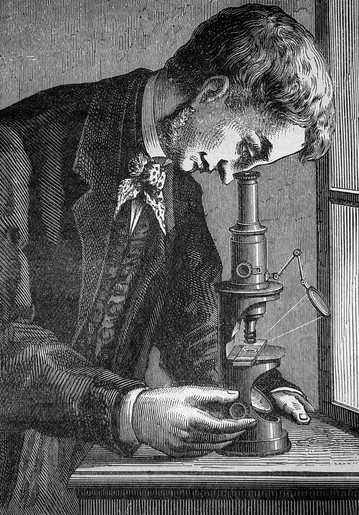
\includegraphics[width=\textwidth]{images/old_microscope.jpg}
		\end{subfigure}
		\begin{subfigure}{0.27\textwidth}
			\centering
			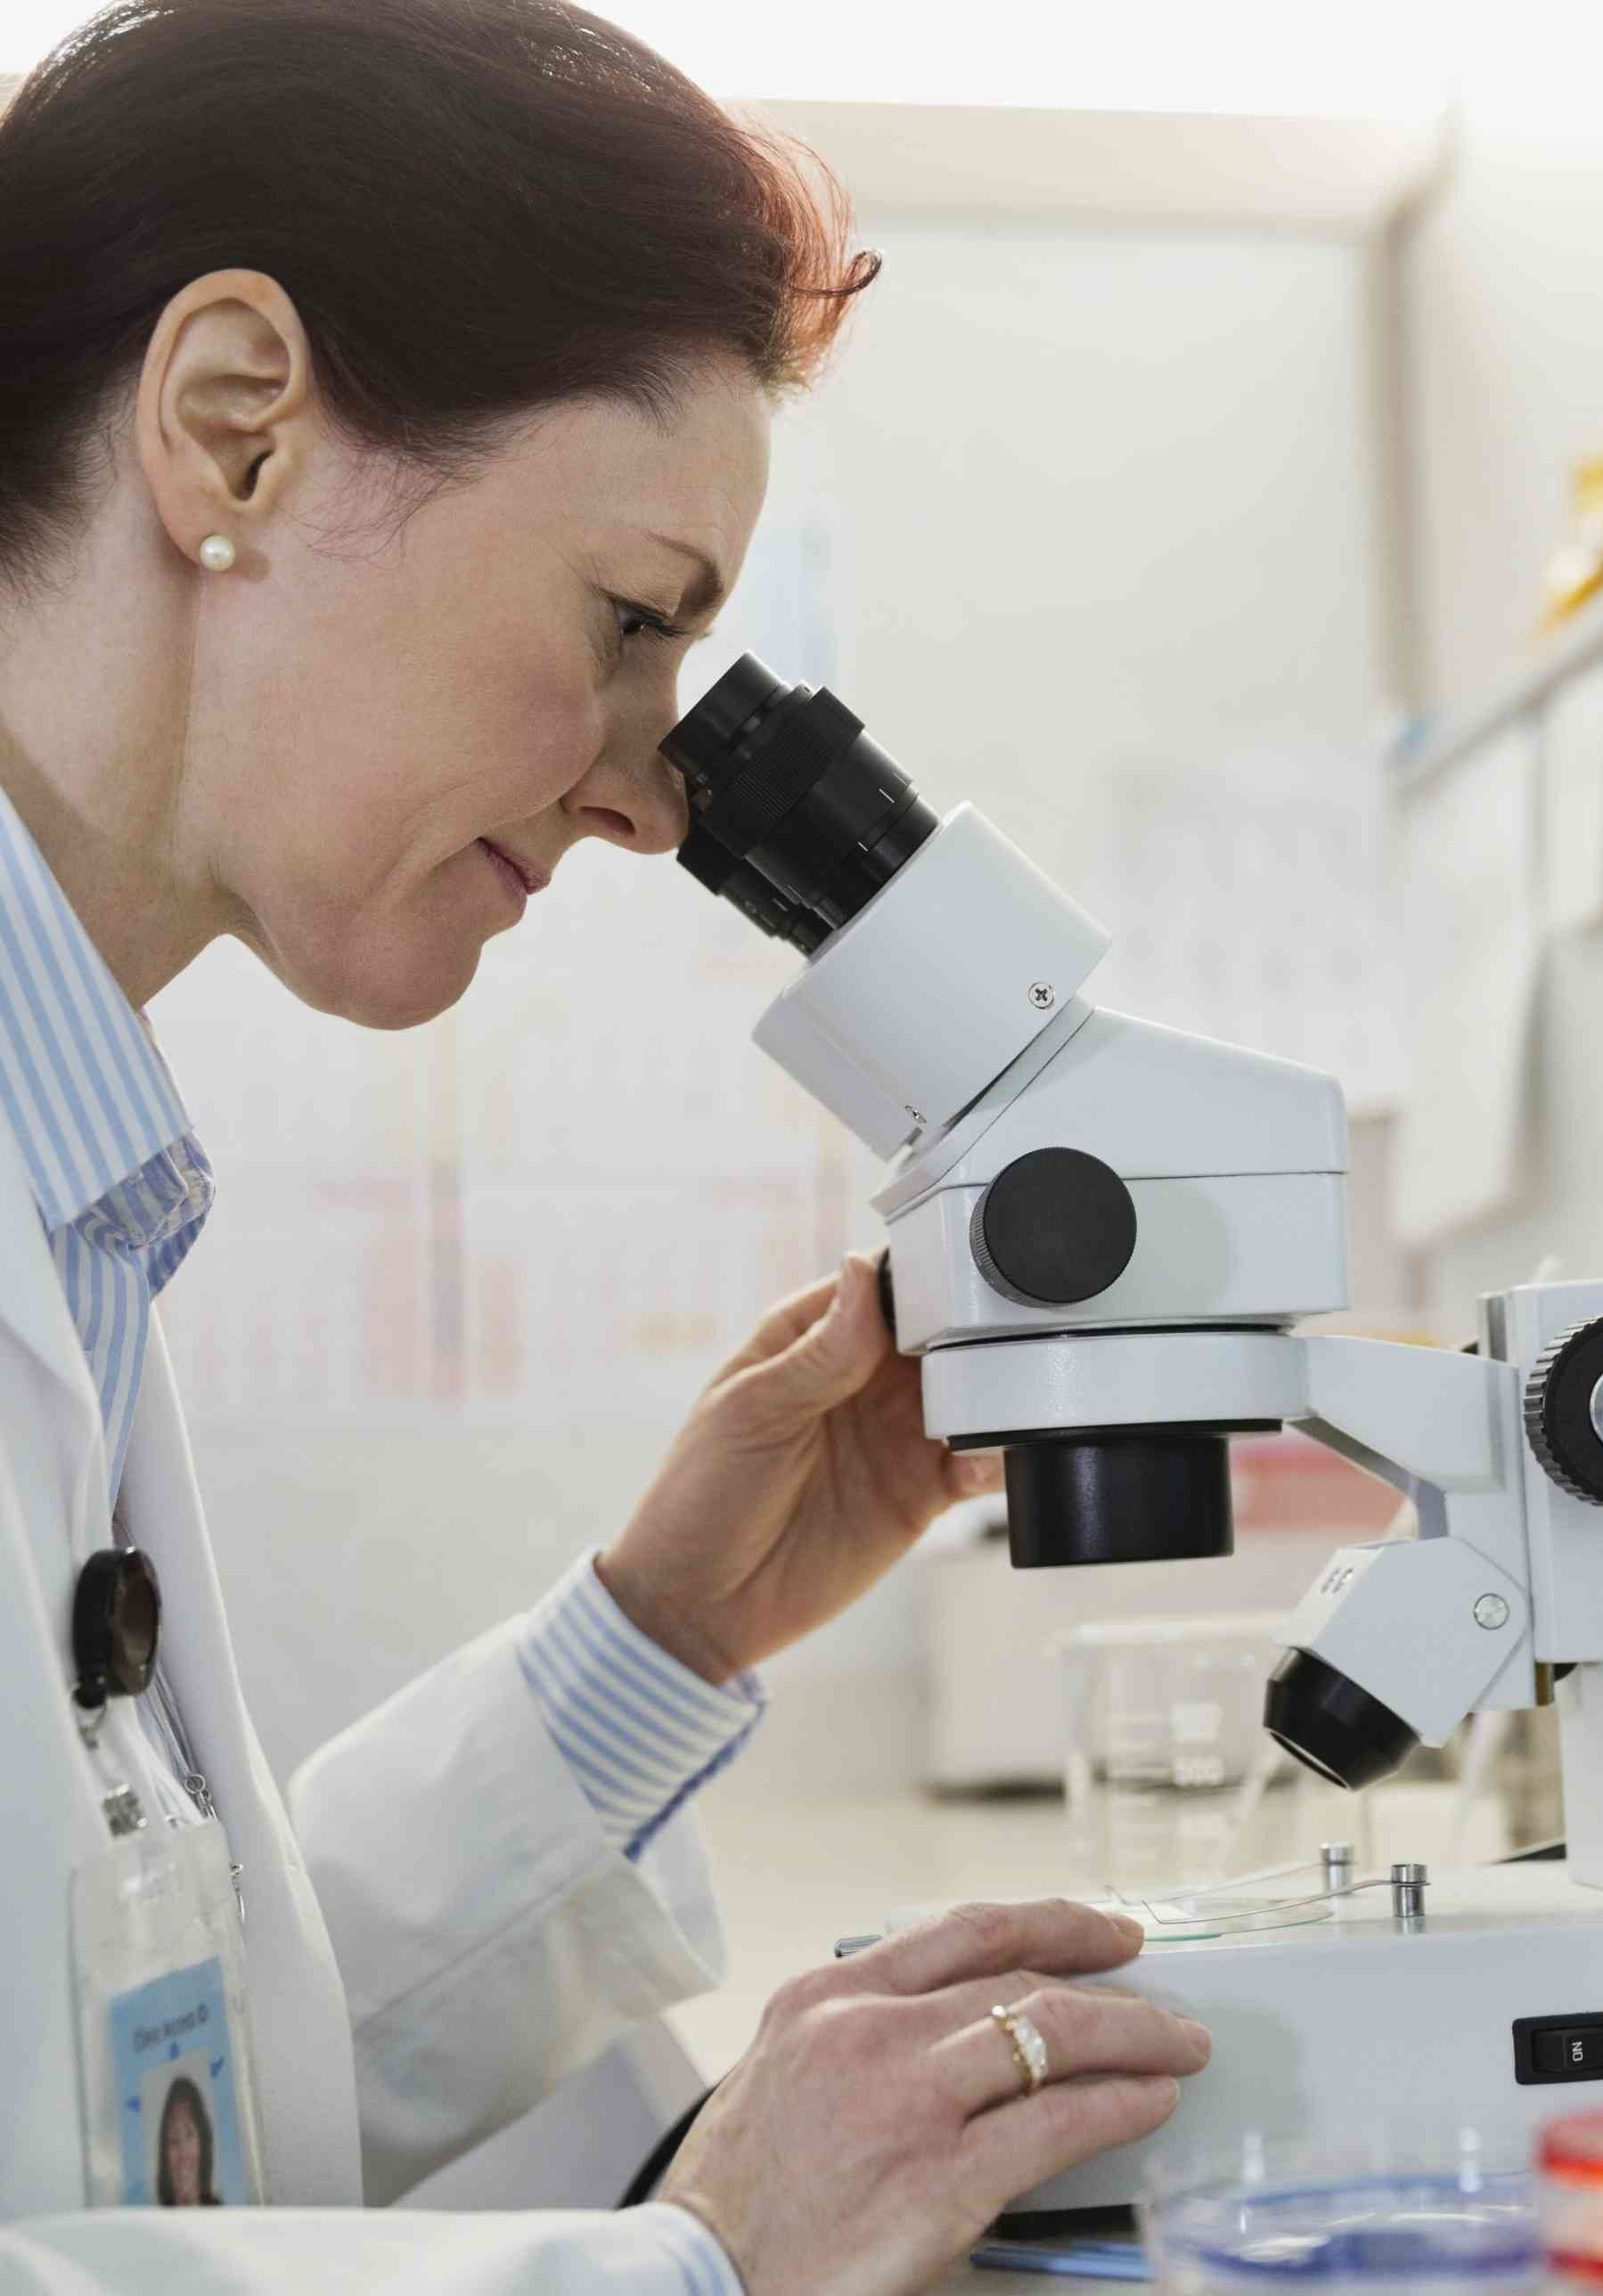
\includegraphics[width=\textwidth]{images/new_microscope.jpg}
		\end{subfigure}
		\begin{subfigure}{0.27\textwidth}
			\centering
			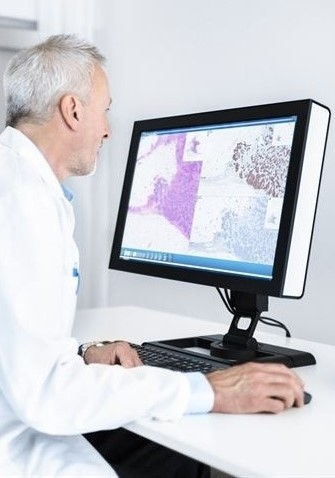
\includegraphics[width=\textwidth]{images/dpath_microscope.jpg}
		\end{subfigure}
	\end{figure}
	\begin{center}
	``\textit{Digital pathology incorporates the acquisition, management, sharing and \textbf{interpretation} of pathology information — including slides and data — in a digital environment}" 
	\end{center}
	\hfill
	{\tiny\textit{left:} institutions.ville-geneve.ch, \textit{center:} verywellhealth.com, \textit{right:} healthcare-in-europe.com}
\end{frame}

\subsection{Pathology workflow}
\begin{frame}{From the body to the computer}
	\vfill

	A pathology workflow: from a biopsy...
	\begin{figure}[h]
		\centering
		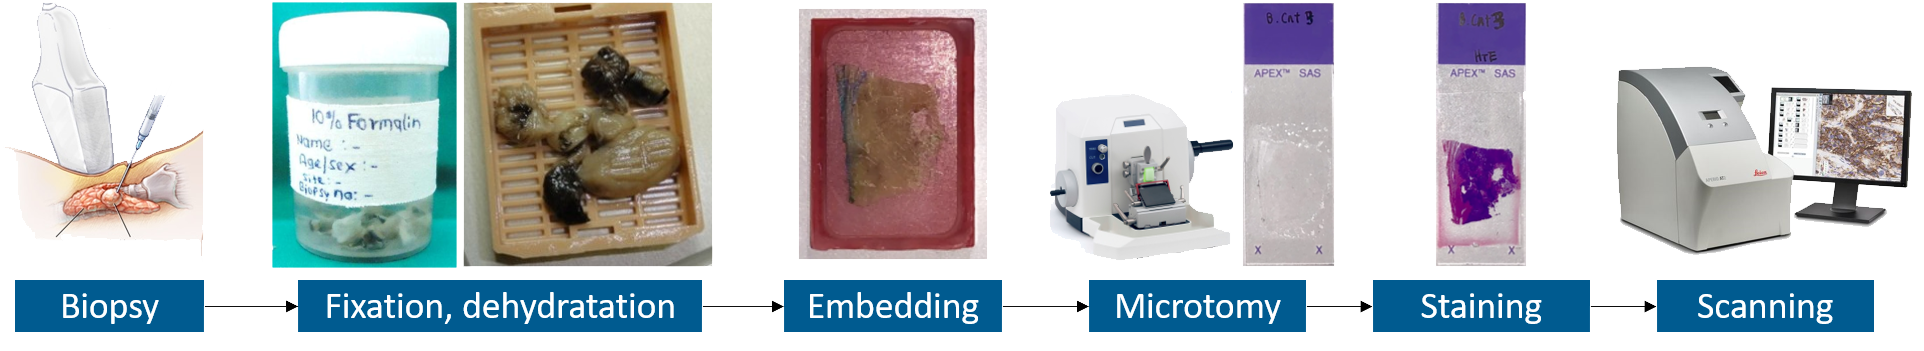
\includegraphics[width=\textwidth]{images/pathology_workflow.png}
	\end{figure}
	
	\vfill
	
	... to a whole-slide image and computer-aided pathology (CAP).
	\begin{figure}
		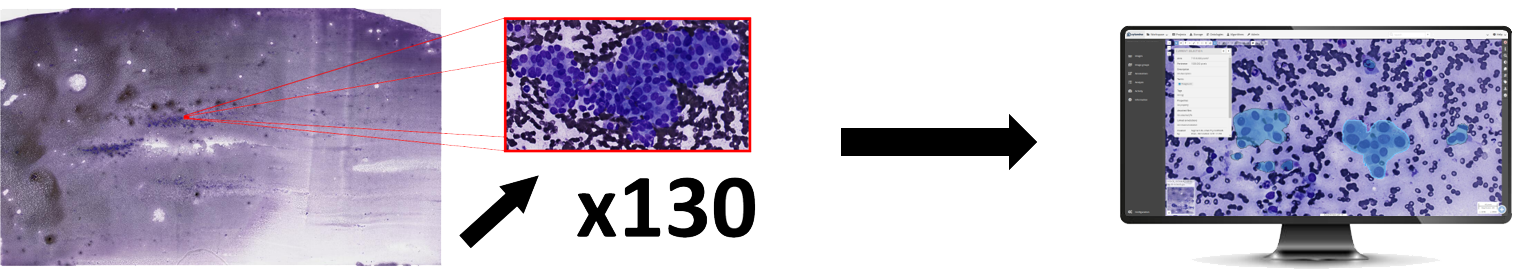
\includegraphics[width=\textwidth]{images/whole-slide-to-cap.png}
		\caption*{\small Left image: 163840 x 95744 pixels$^2$, 2.3 Gb.}
	\end{figure}
	
	\vfill
\end{frame}

\subsection{Computer-aided pathology}
\begin{frame}{Why computer-aided pathology}

\vfill

\begin{center} Some pathology analysis tasks are \textbf{tedious}, \textbf{time-consuming} and are subject to \textbf{inter/intra-observer variabilities}. \end{center} 

\vfill

\begin{figure}
	\begin{subfigure}{0.25\textwidth}
		\centering
		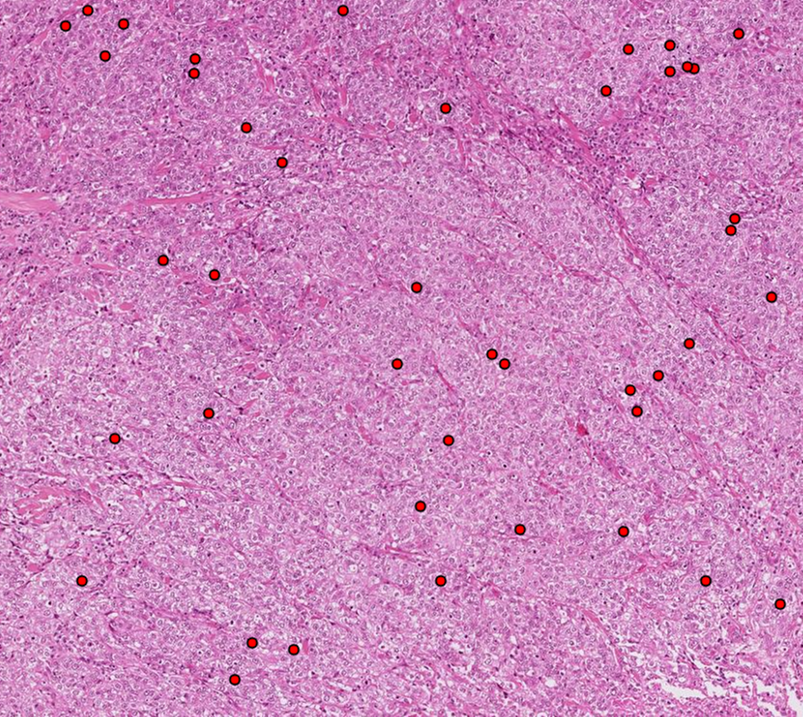
\includegraphics[width=\textwidth]{images/mitosis_zoomout.png}
		\caption{Counting}
	\end{subfigure}
	\begin{subfigure}{0.28\textwidth}
		\centering
		\vfill
		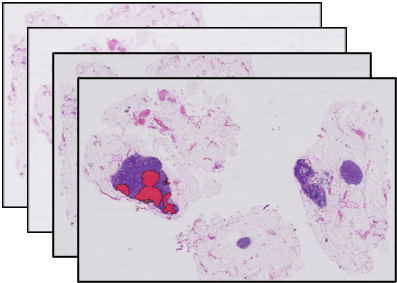
\includegraphics[width=\textwidth]{images/highdatavolume.png}
		\vfill
		\caption{Multi-slide analysis}
	\end{subfigure}
	\begin{subfigure}{0.45\textwidth}
		\centering
		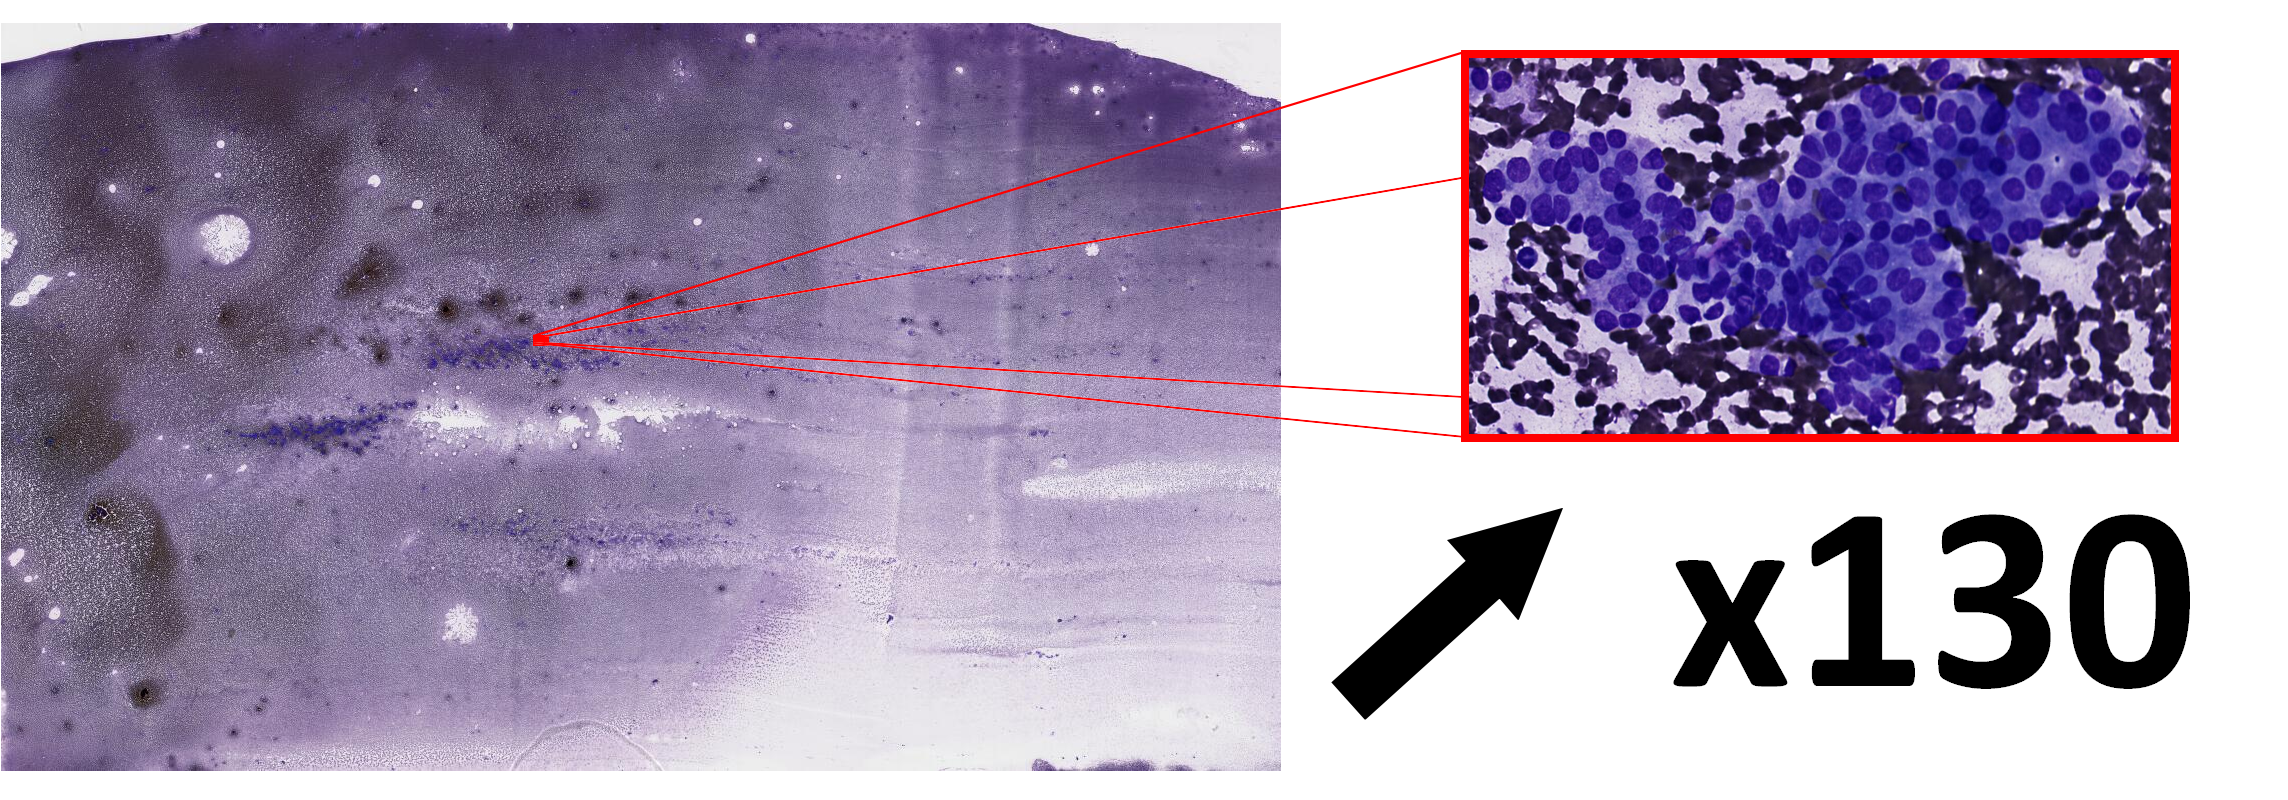
\includegraphics[height=0.2\textheight]{images/whole-slide-dim.png}
		\caption{Needle in a haystack}
	\end{subfigure}
\end{figure}
\vfill 
\begin{center}
Computational methods can improve analysis \textbf{reliability and speed} therefore \textbf{improving patient outcome and costs}. 
\end{center}
\vfill
\end{frame}

\begin{frame}{Cytomine}
\end{frame}

\begin{frame}{Using machine and deep learning}
	\begin{center}
	Machine learning methods are often preferred to classical computer vision methods for tackling complex pathology tasks.
	\end{center}
	\vfill
	\begin{figure}
		\centering
		\begin{subfigure}{0.32\textwidth}
			\centering
			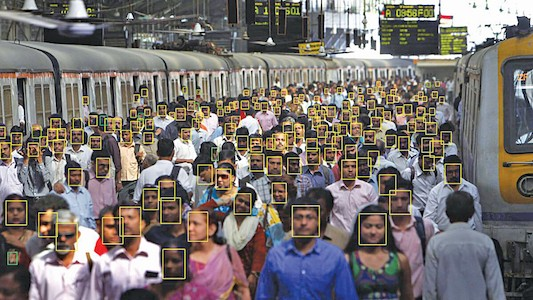
\includegraphics[width=\textwidth]{images/facedetect.jpg}
		\end{subfigure}
		\begin{subfigure}{0.32\textwidth}
			\centering
			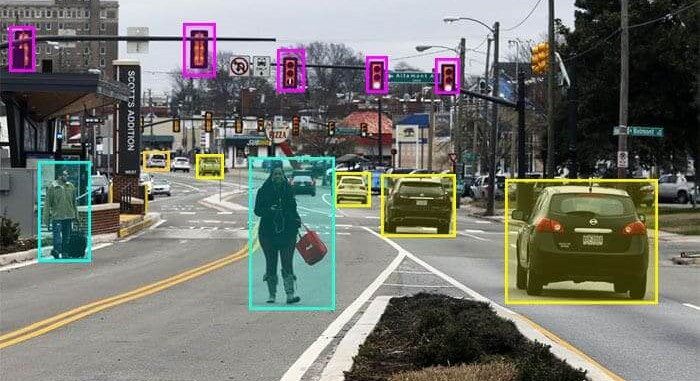
\includegraphics[width=\textwidth]{images/bounding-boxes.jpg}
		\end{subfigure}
		\begin{subfigure}{0.32\textwidth}
			\centering
			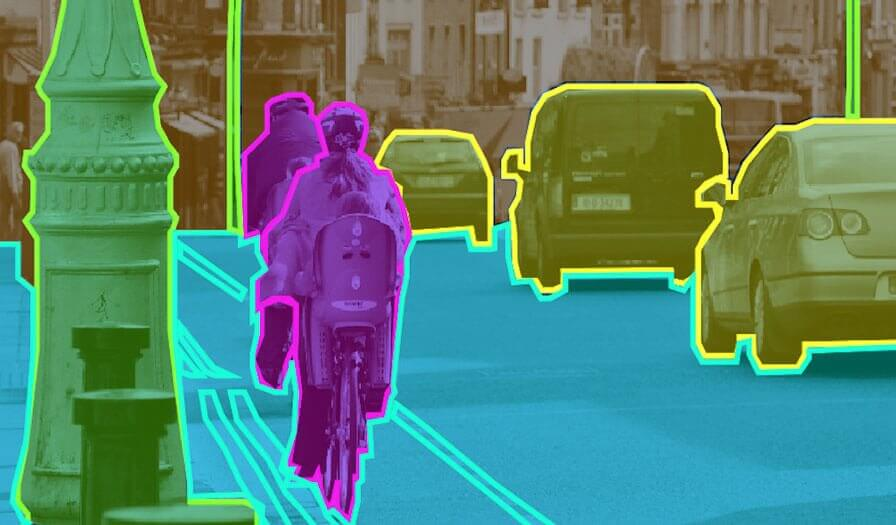
\includegraphics[width=\textwidth]{images/segment_sgment.jpg}
		\end{subfigure}
	\end{figure}
	\vfill
	\begin{center}
		\textbf{Deep learning methods} are particularily \textbf{efficient for computer vision} problems and have seen a surge of interest from the CAP community.  
	\end{center}
	\begin{figure}
		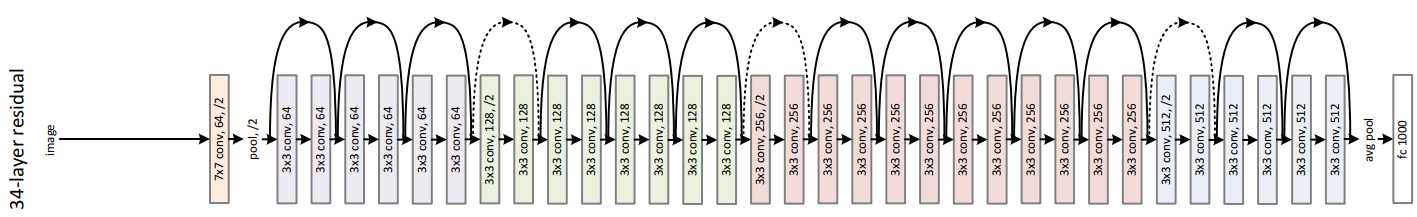
\includegraphics[width=\textwidth]{images/resnet34.png}
	\end{figure}
\end{frame}

\begin{frame}{Computer-aided pathology is challenging}
	Few of the challenges:
	\begin{itemize}
		\item {high variability}: slide preparation process, artefacts, staining, acquisition,...
		\item {big data}: up to millions of biological objects per multi-gigapixel image
		\item {data scarcity}: annotating data is expensive and tedious
	\end{itemize}
\end{frame}

\subsection{Data scarcity}
\begin{frame}[t]{Data scarcity in digital pathology}
	\vspace{0.5cm}

	\begin{quotation}
		``\textit{We are drowning in information but starving for knowledge.}'' {\footnotesize Rutherford D. Roger}
	\end{quotation}

	\vfill

	\begin{figure}
		\begin{subfigure}{0.32\textwidth}
			\centering
			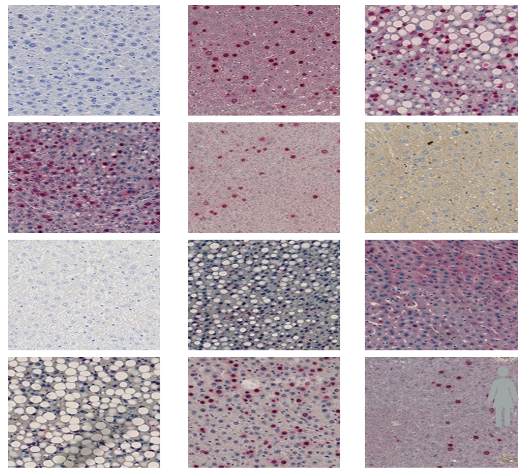
\includegraphics[width=\textwidth]{images/variability.png}
			\caption*{\tiny Variability}
		\end{subfigure}
		\hfill
		\begin{subfigure}{0.32\textwidth}
			\centering
			
\includegraphics[width=\textwidth]{images/gdpr.png}
			\caption*{\tiny Privacy}
		\end{subfigure}
		\hfill
		\begin{subfigure}{0.32\textwidth}
			\centering
			
\includegraphics[width=0.9091\textwidth]{images/graduate.png}
			\caption*{\tiny Need for skilled annotators}
		\end{subfigure}
		% \hfill
		% \begin{subfigure}{0.25\textwidth}
		% 	\centering
		% 	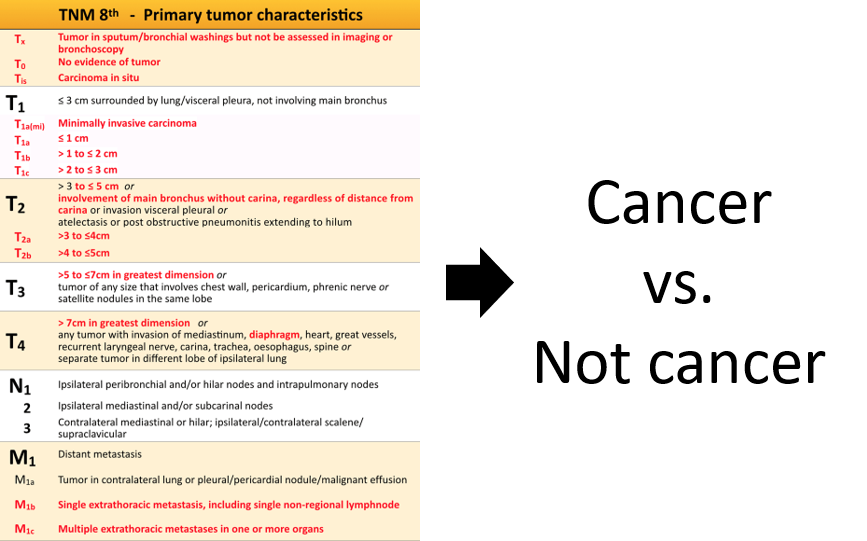
\includegraphics[width=\textwidth]{images/simplification.png}
		% 	\caption*{\tiny Task simplification}
		% \end{subfigure}
	\end{figure}

\end{frame}
\begin{frame}{Natural images \textit{vs.} pathology datasets}
	\vspace{-0.5cm}
	\begin{columns}
		\column{.25\linewidth}
		\begin{figure}
			\centering
			\caption*{\footnotesize \textbf{Natural images}}
			\vspace{-0.25cm}
			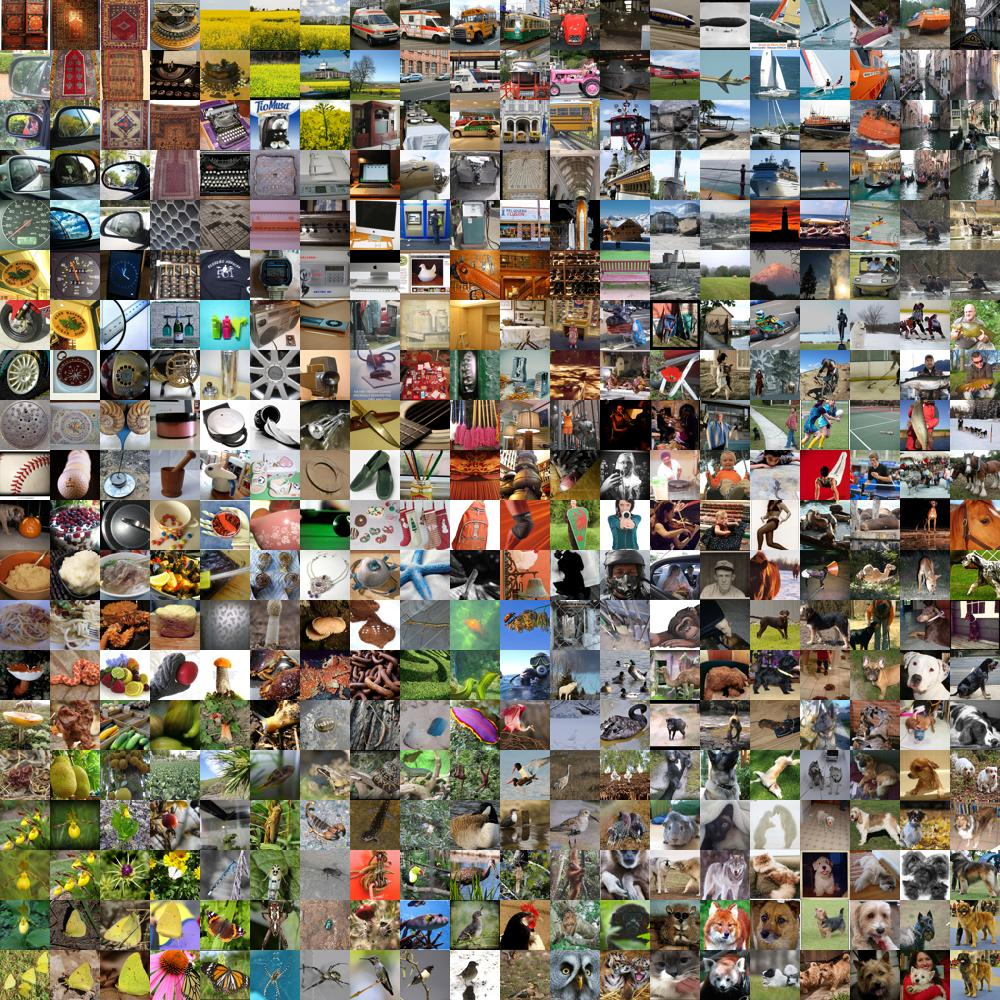
\includegraphics[width=\textwidth]{images/illuimagenet.jpg}
		\end{figure}
		\column{.4\linewidth}
		{%
\vfill
\footnotesize \noindent ImageNet \parencite{deng2009imagenet}:
\begin{itemize}
\item \textbf{Task}: classif.
\item \textbf{Images}: $1.3$M images (now $14$M)
\item \textbf{Annot.}: one label/image
\item \textbf{Classes}: 1000
\end{itemize}
\vfill
		}
		
	\end{columns}
	\begin{columns}
		\column{.25\linewidth}
		\begin{figure}
			\centering
			\caption*{\footnotesize \textbf{Pathology images}}
			\vspace{-0.25cm}
			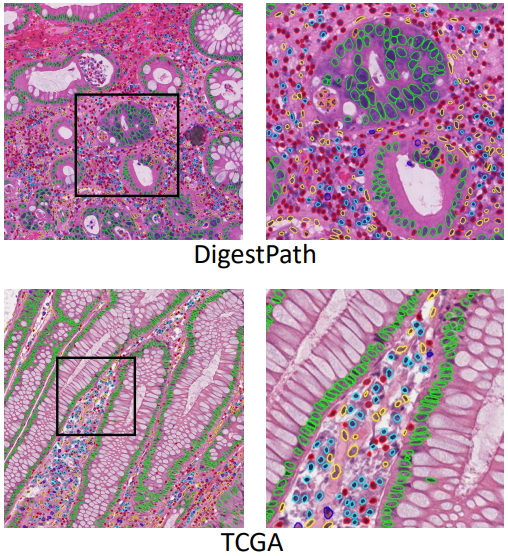
\includegraphics[width=\textwidth]{images/lizard.png}
		\end{figure} 
		\column{.4\linewidth}
		{%
\vfill
\footnotesize \noindent Lizard \parencite{graham2021lizard}:%
\begin{itemize}
	\item \textbf{Task}: classif/seg
	\item \textbf{Images}: 291 images/regions
	\item \textbf{Annot.}: 500k nuclei
	\item \textbf{Classes}: 6
\end{itemize}
\vfill
		}
	\end{columns}

% Consequences:
% \begin{itemize}
% 	\item small datasets (compared to natural image domain)
% 	\item lack of variety on the problem targets 
% 	\item weakly- or sparsely-labeled datasets 
% \end{itemize}
\end{frame}

\begin{frame}{Working around data scarcity}
% 	\textbf{Option 1}: make labeling more efficient.
% 	\vfill
% 	\begin{columns}
% 	\begin{column}[t]{0.33\linewidth}
% 		\begin{figure}
% 			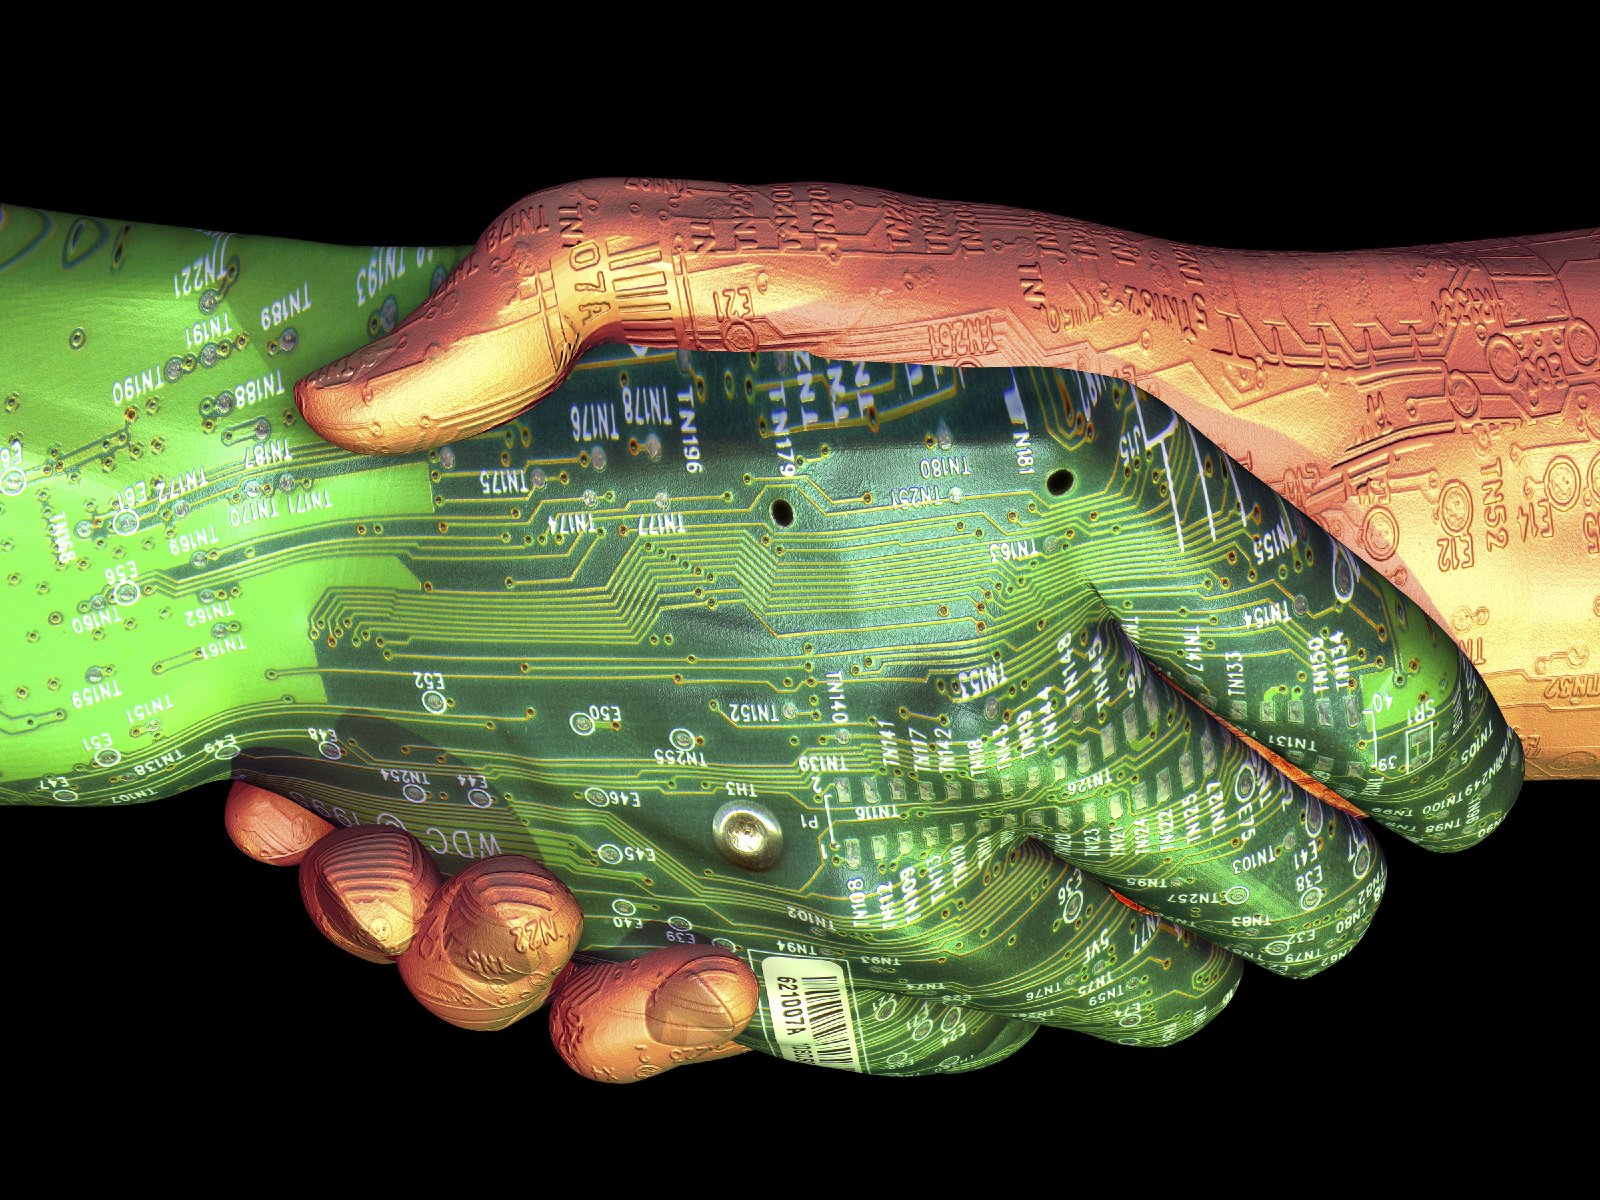
\includegraphics[width=0.9\textwidth]{images/haii.jpg}
% 			\caption*{AI-assisted labeling}
% 		\end{figure}
% 	\end{column}
% 	\hfill
% 	\begin{column}[t]{0.33\linewidth}
% 		\begin{figure}
% 			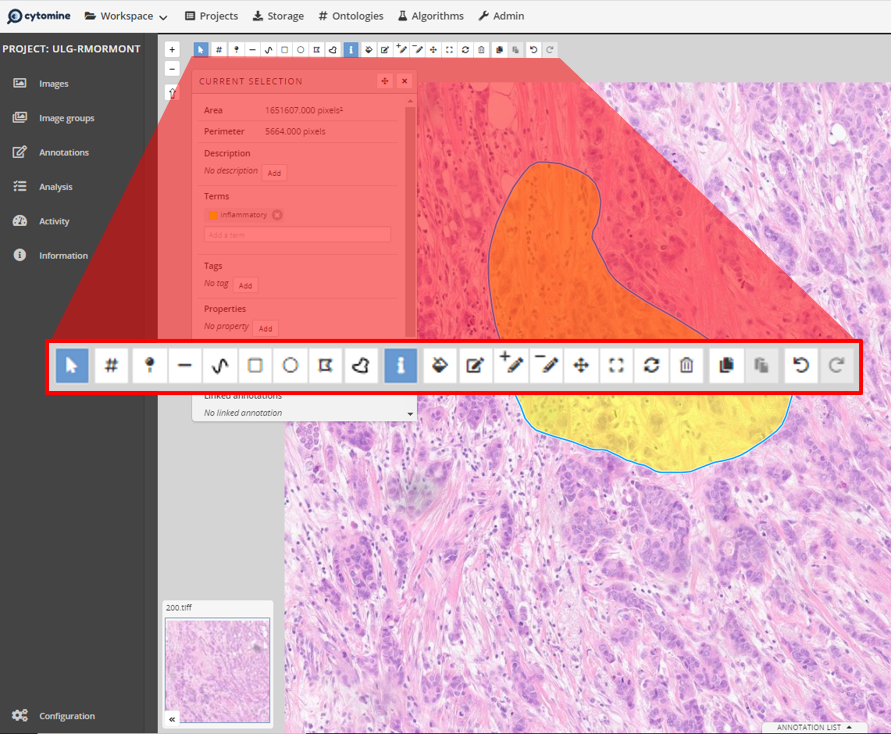
\includegraphics[width=0.9\textwidth]{images/drawing_tools.png}
% 			\caption*{AI-assisted labeling}
% 		\end{figure}
% 	\end{column}
% 	\hfill
% 	\begin{column}[t]{0.33\linewidth}
% 		\begin{figure}
% 			
\includegraphics[width=0.9\textwidth]{images/crowdsourcing.jpg}
% 			\caption*{Crowdsourcing}
% 		\end{figure}
% 	\end{column}
% \end{columns}

\begin{figure}
	\begin{subfigure}{\linewidth}
		\centering
		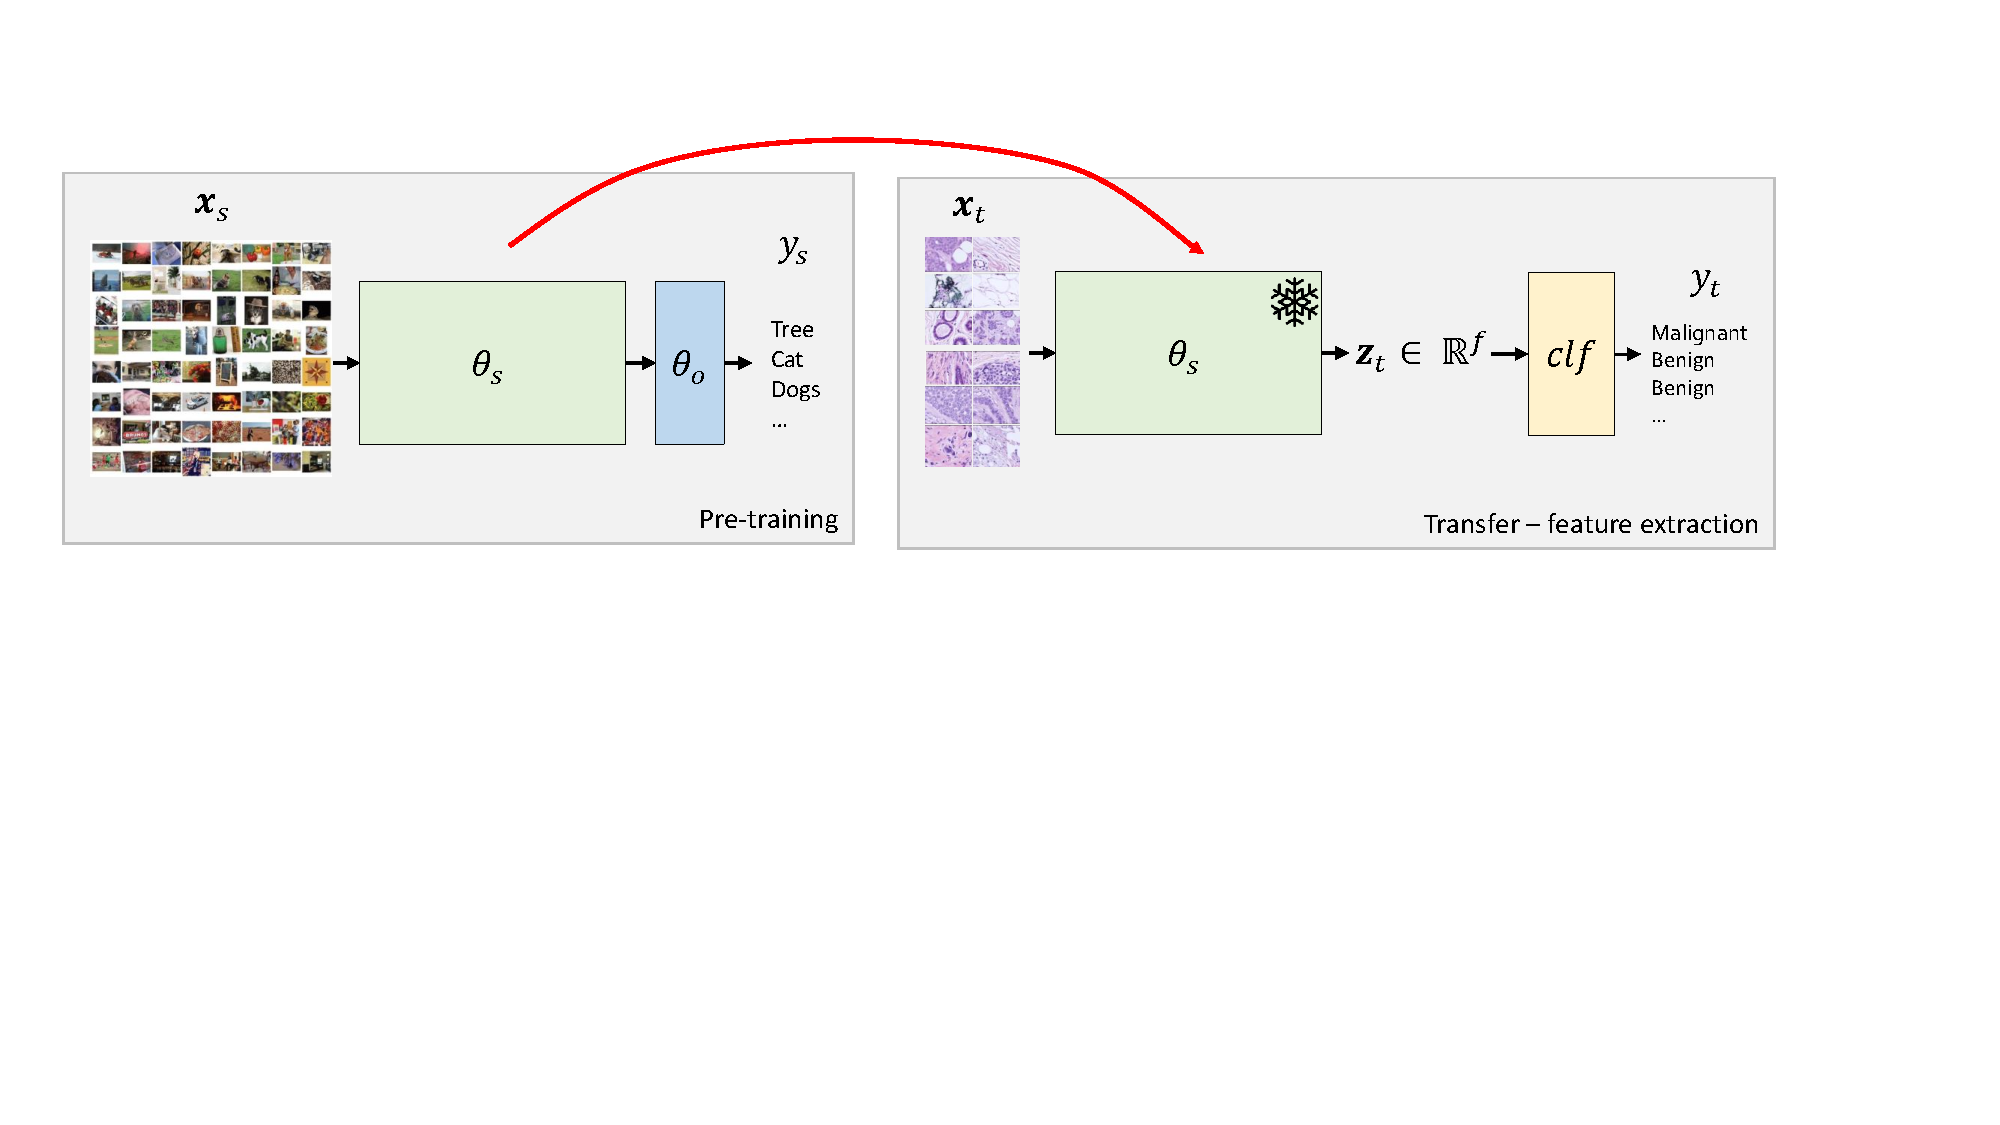
\includegraphics[width=0.7\textwidth]{images/transfer-fe.pdf}
		\caption*{Transfer learning}
	\end{subfigure}

	\begin{subfigure}{\linewidth}
		\centering
		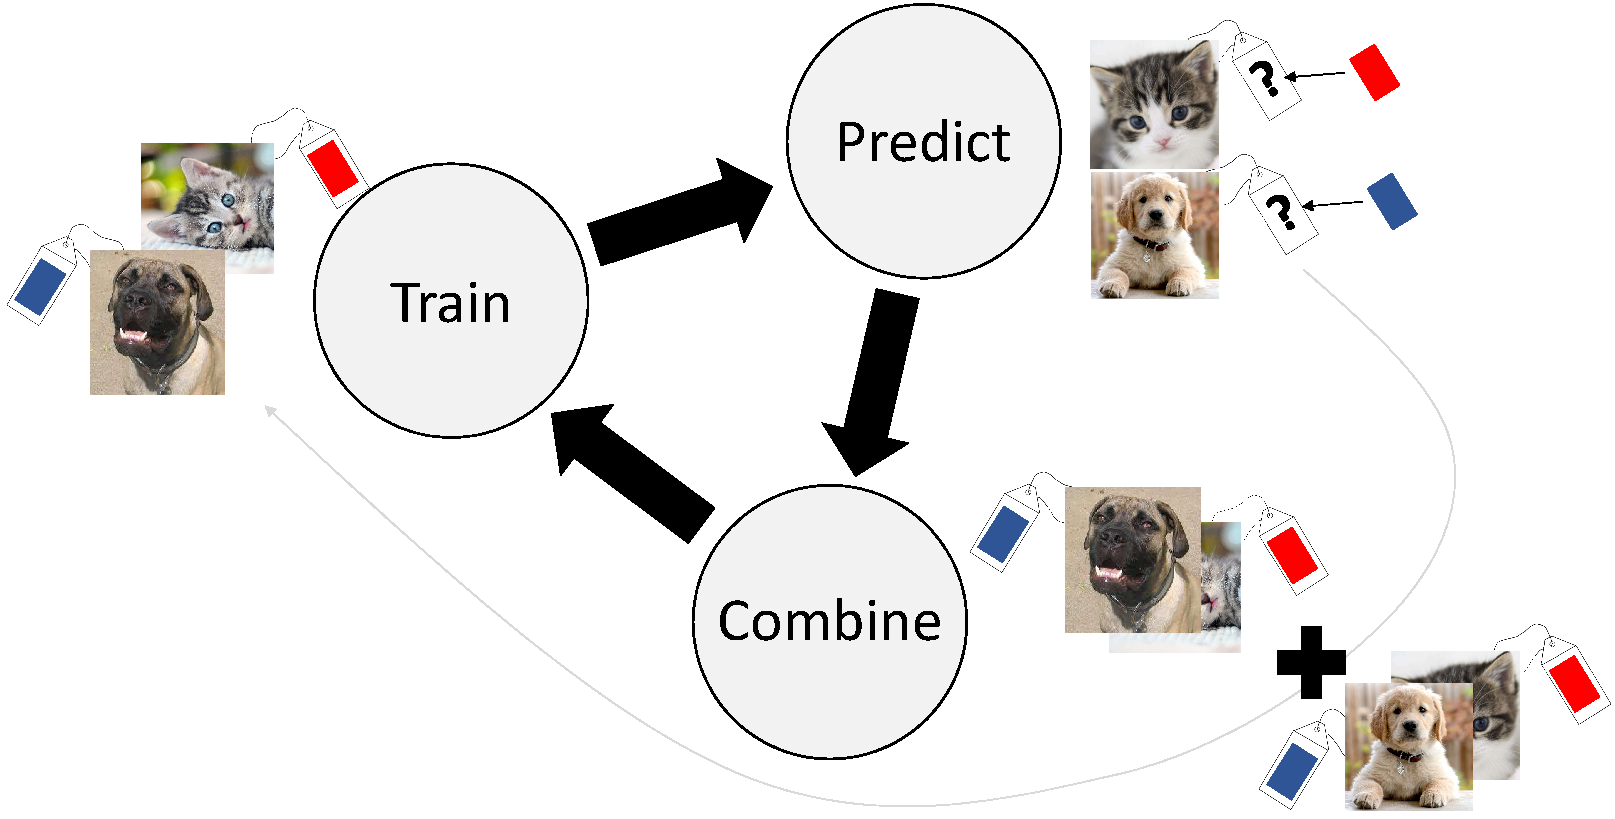
\includegraphics[width=0.7\textwidth]{images/selftraining.pdf}
		\caption*{Self-training}
	\end{subfigure}
\end{figure}
\end{frame}

\subsection{Outline}
\begin{frame}{Outline}
	\vfill
	Contributions:
	\begin{enumerate}
		\item \textbf{Transfer from ImageNet}
		\begin{figure}
			\centering
			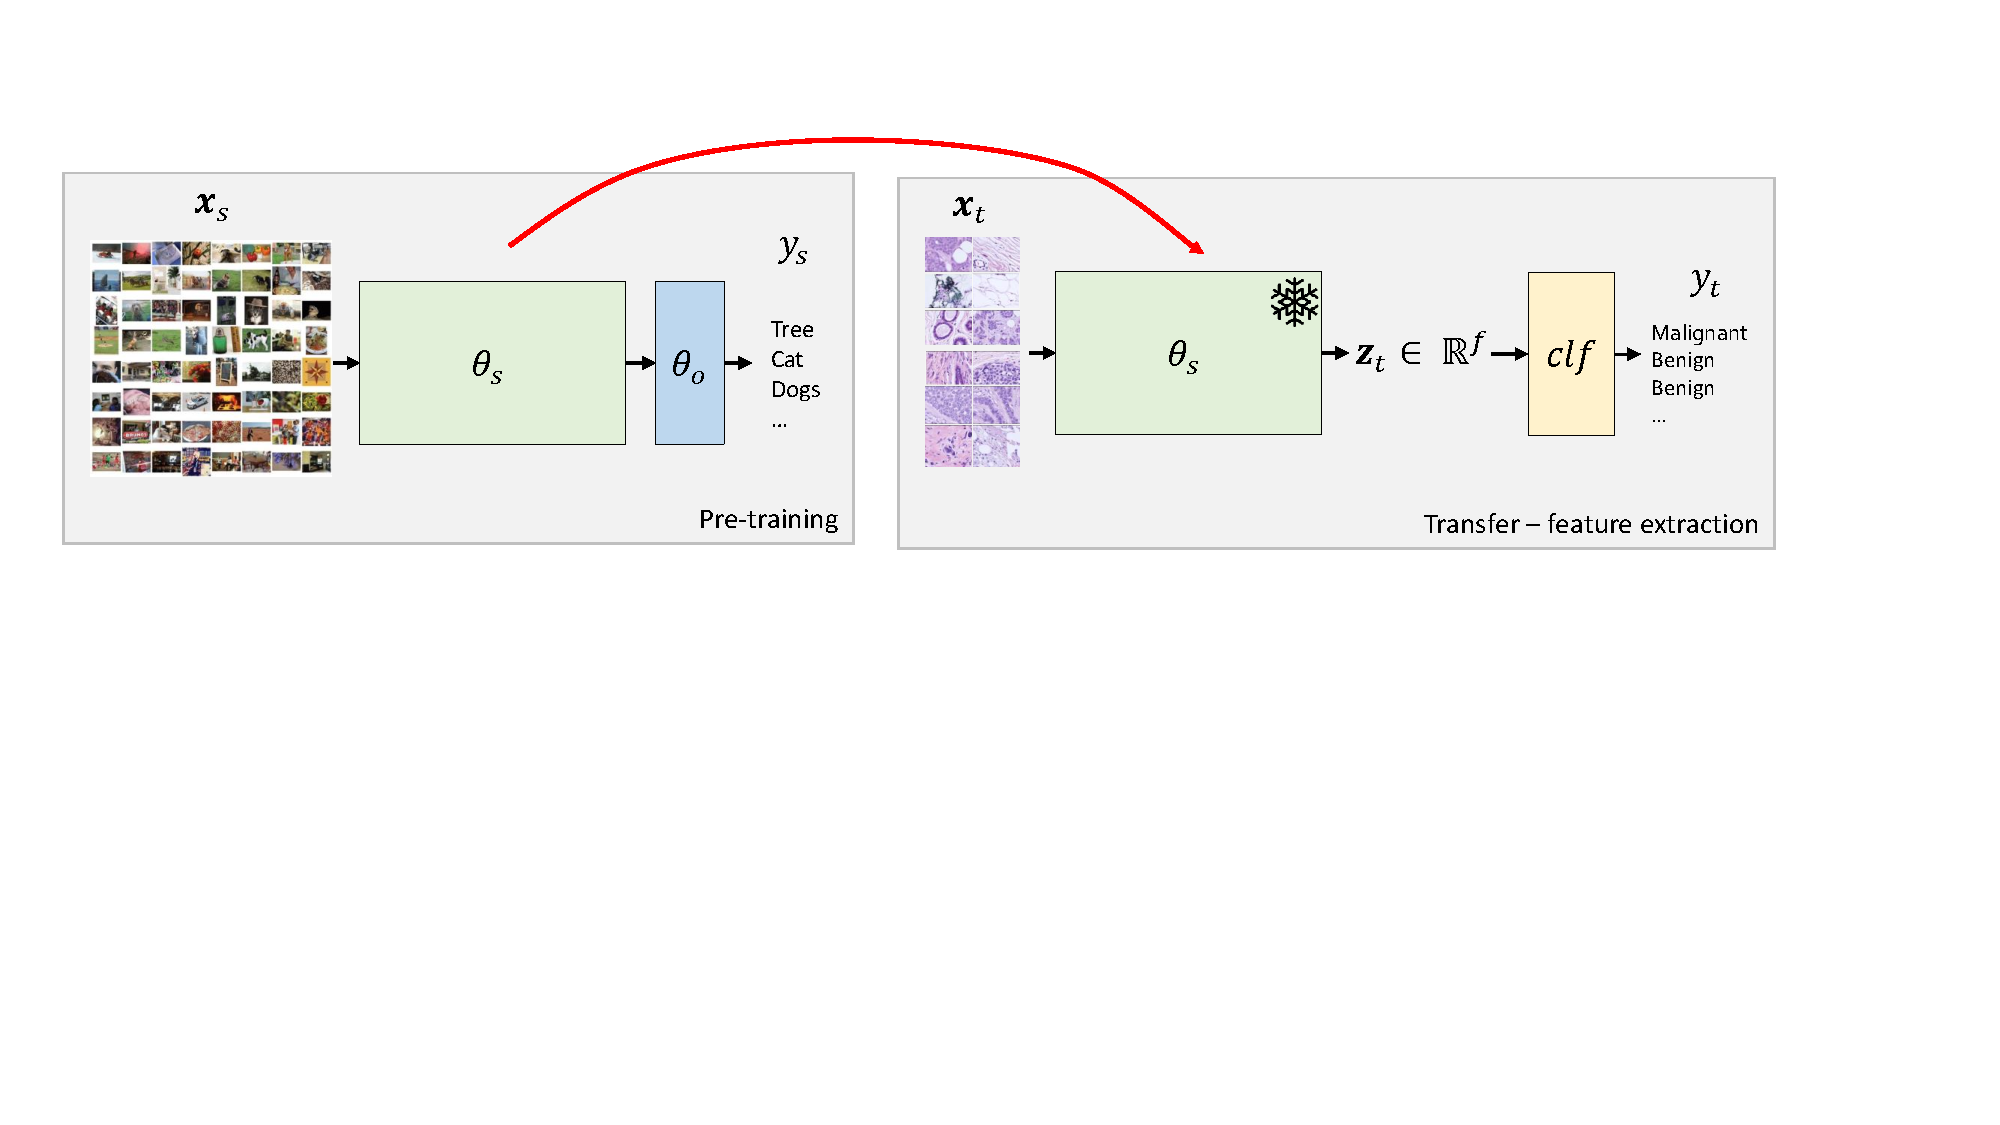
\includegraphics[height=0.15\textheight]{images/transfer-fe.pdf}
		\end{figure}
		\item \textbf{Transfer from pathology data}
		\begin{figure}
			\centering
			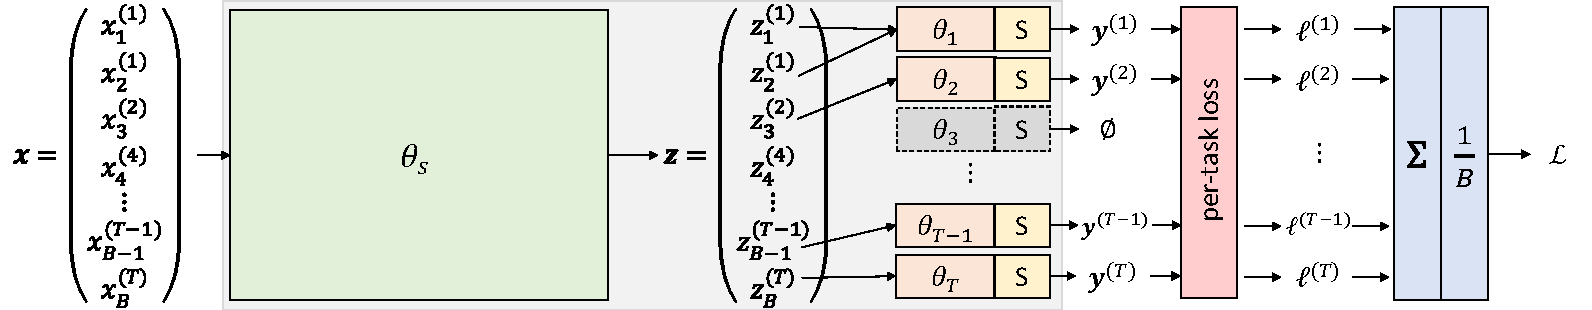
\includegraphics[height=0.15\textheight]{images/multitask-training.pdf}
		\end{figure}
		\item \textbf{Self-training for segmentation from sparsely-labeled data}
		\begin{figure}
			\centering
			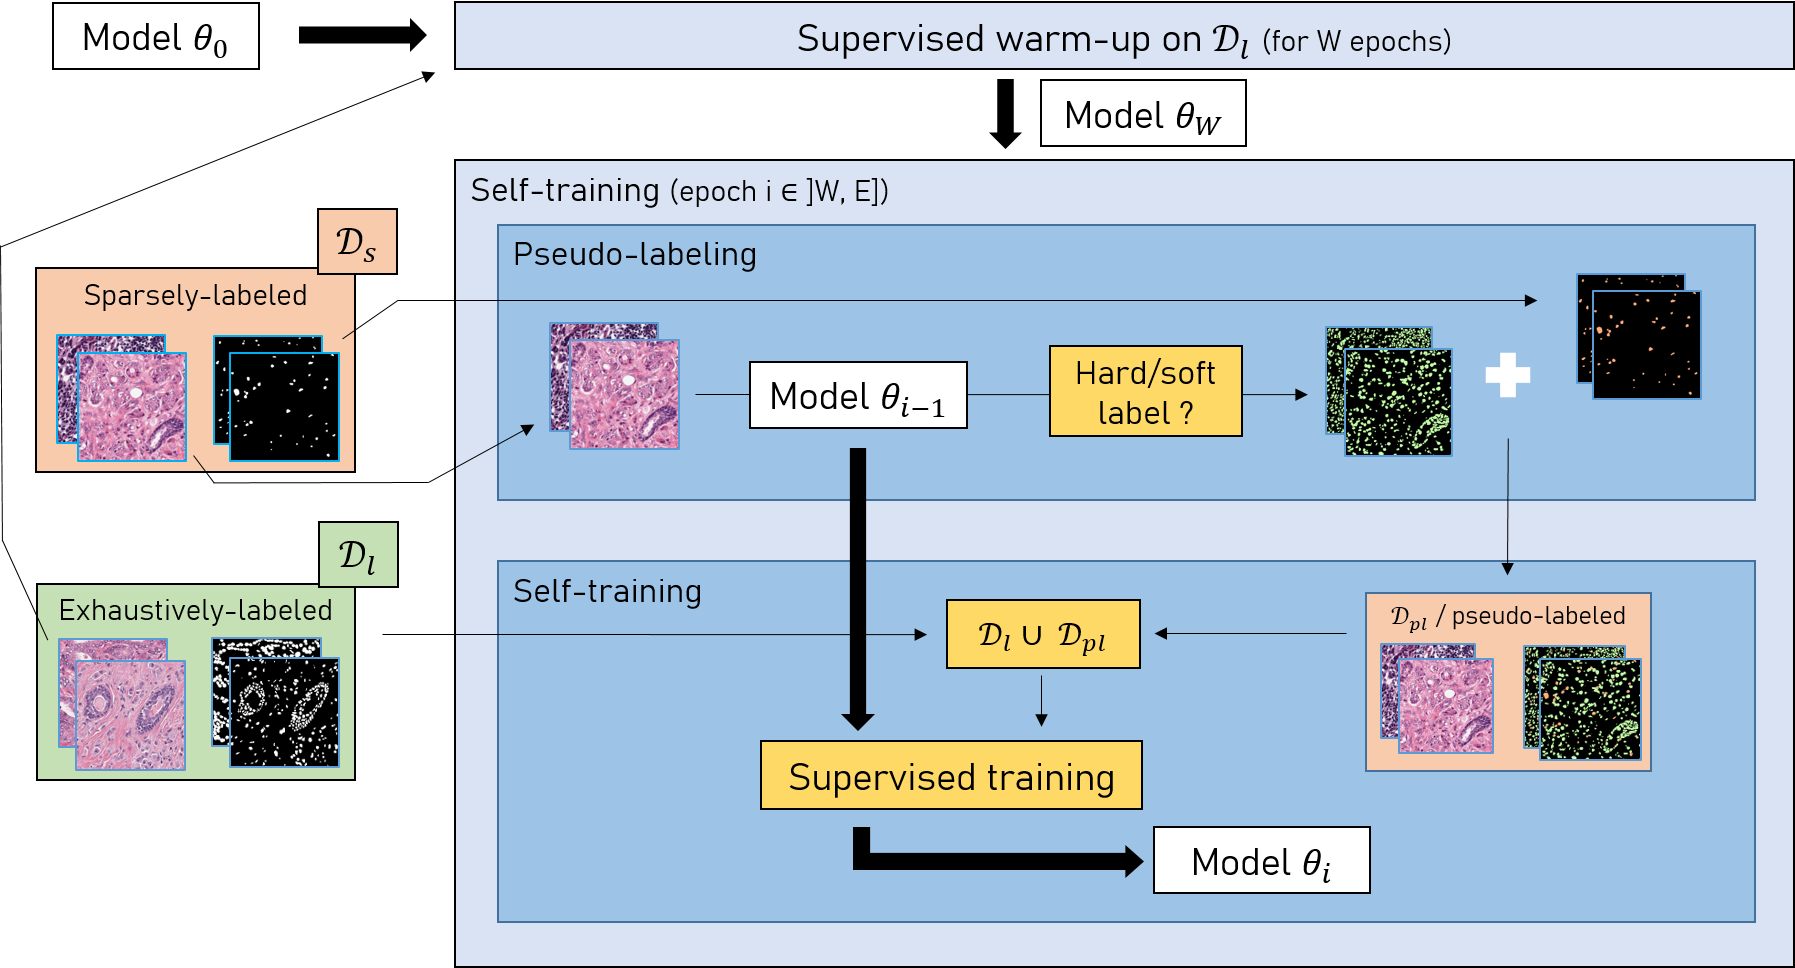
\includegraphics[height=0.2\textheight]{images/selftrain-algo.png}
		\end{figure}
	\end{enumerate}
	\vfill
\end{frame}

\section{Transfer from ImageNet}
\subsection{Introduction}

\begin{frame}{}
	\vfill
	\begin{center}
		\Large
		Contribution \#1 \\
		\vspace{0.75cm}
		\textbf{Transfer learning from ImageNet} \\
		\vspace{0.75cm}
		{\small (thesis chapter 4)}
	\end{center}
	 
	\vfill

	{
		\footnotesize
		\textbf{Article}: \fullcite{mormont2018comparison}
	}	
\end{frame}

\begin{frame}{Deep transfer learning: how to?}
	\begin{figure}
		\centering
		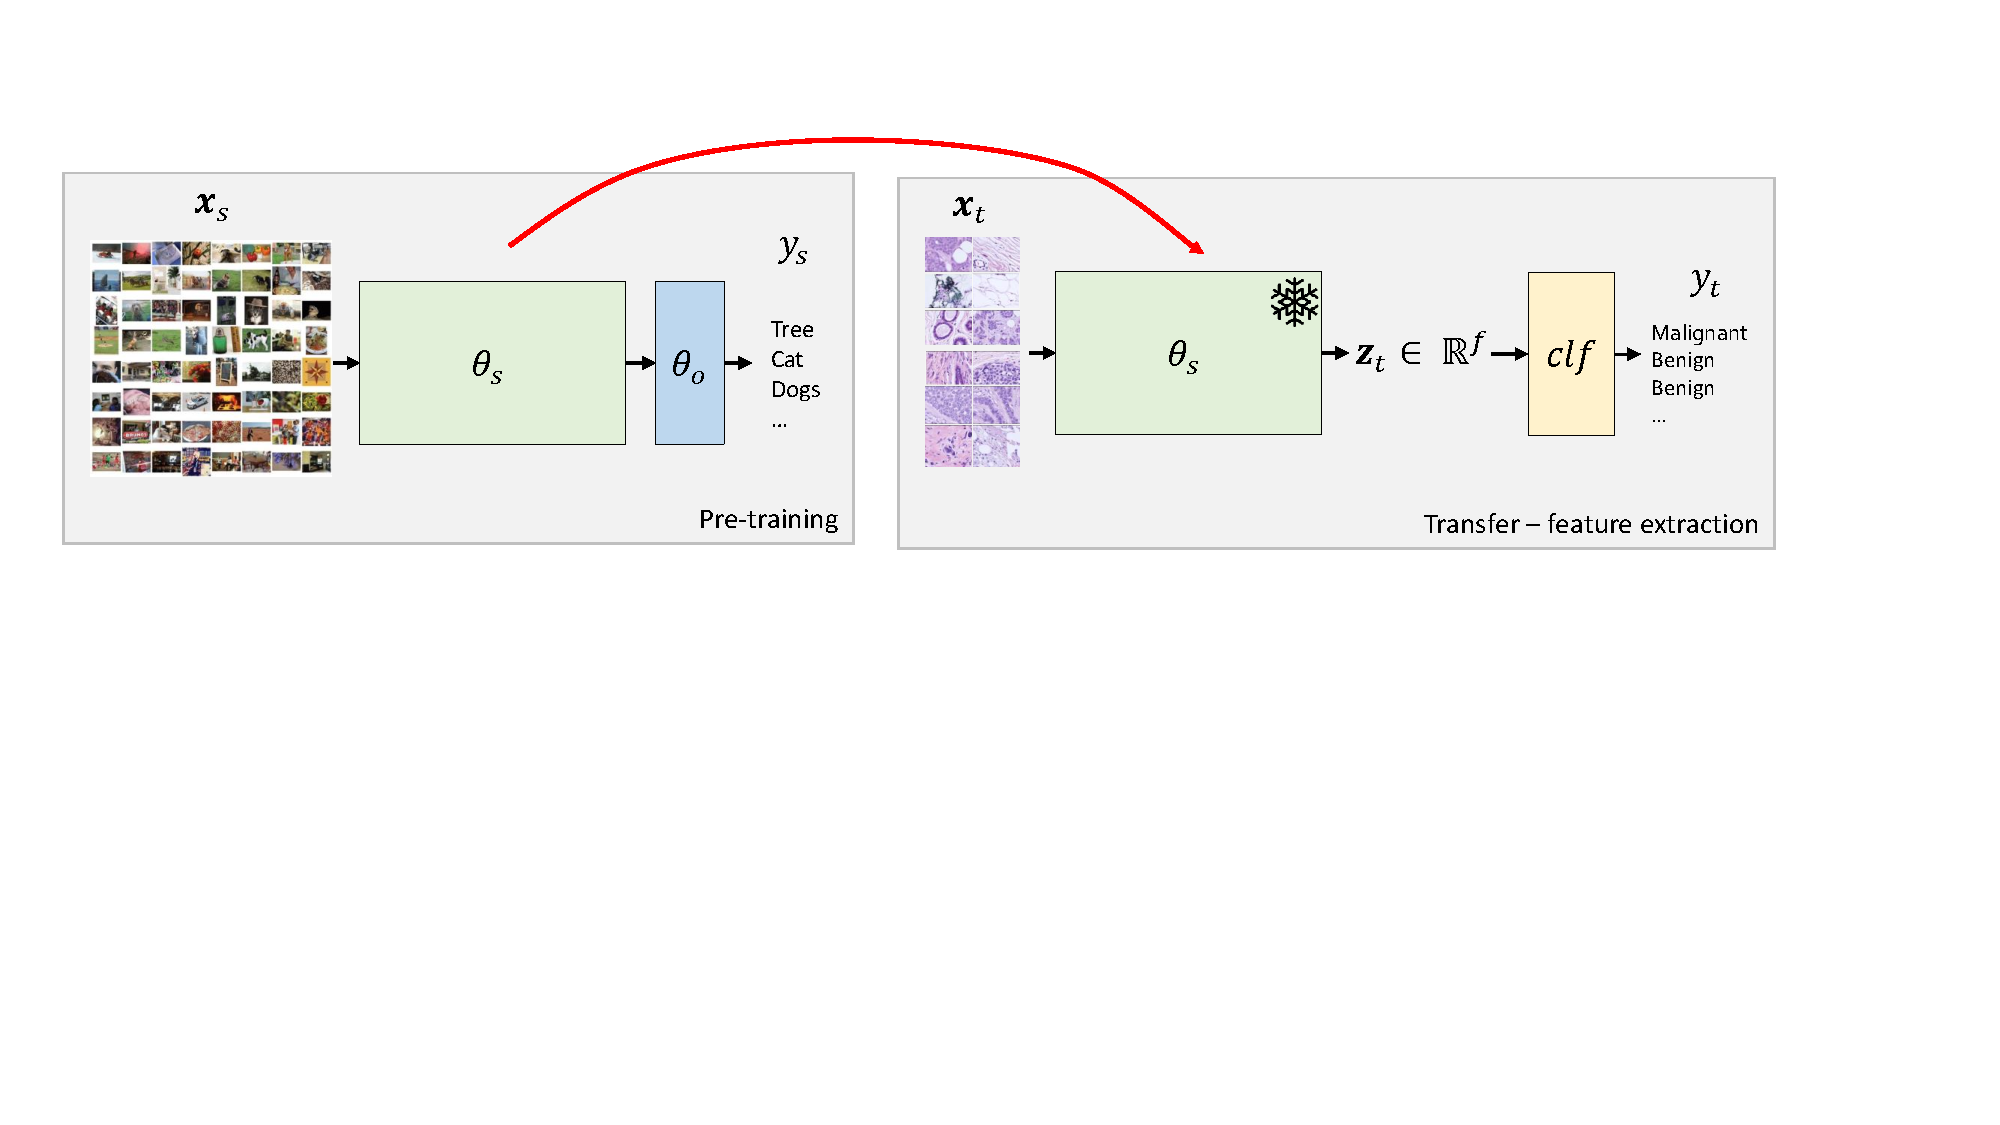
\includegraphics[width=0.9\textwidth]{images/transfer-fe.pdf}
		\caption*{Feature extraction}
	\end{figure}
	\begin{figure}
		\centering
		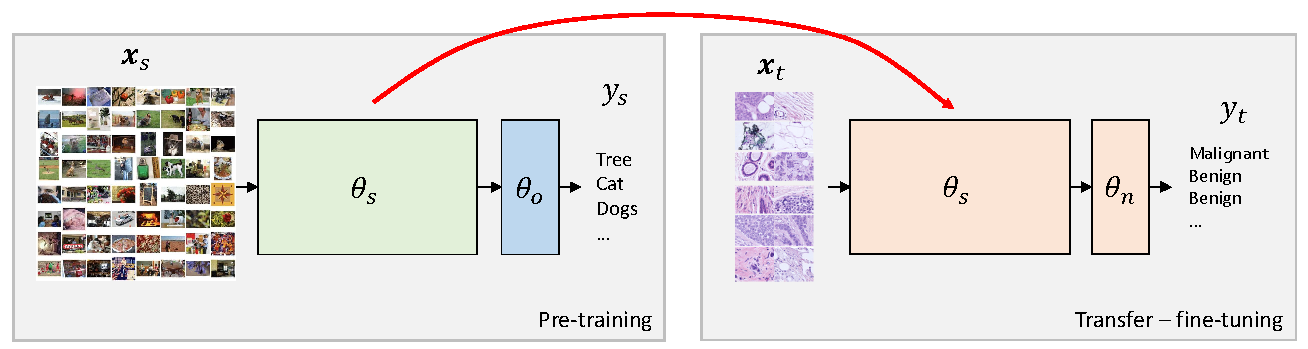
\includegraphics[width=0.9\textwidth]{images/transfer-ft.pdf}
		\caption*{Fine tuning}
	\end{figure}
\end{frame}

\begin{frame}{Our contribution}

\textbf{Goal}: devise \textbf{guidelines and best practices} for deep transfer learning with \textbf{ImageNet as a source task} in \textbf{digital pathology}:

\vfill

\begin{itemize}
	\item {Fine-tuning \textit{vs.} feature extraction}: which one works better ? 
 	\item Which {pre-trained architecture} works better ? {\tiny (ResNet, DenseNet, VGG...)}
 	\item {Where to extract} features ? {\tiny (last layer, inside the network)}
 	\item ...
\end{itemize} 

% \vfill
% We have carried out several experiments \textbf{with ImageNet} as source task:
% \vfill
% \begin{itemize}
% 	 \item \textbf{Feature extraction} vs. \textbf{fine-tuning}
% 	 \item \textbf{Networks}: ResNet50, DenseNet201, VGG16/19, InceptionResNetV2, \textit{etc}.
% 	 \item \textbf{Features classifiers}: SVM , extra-trees (ET), \textit{etc}.
% 	 \item Feature extraction at {increasing depth}
% 	 \item Feature relevance evaluation
% \end{itemize}
\end{frame}


\subsection{Data}
\begin{frame}{Datasets}
8 image classification datasets. 

\begin{table}
    \center 
    \tiny
    \begin{tabular}{|c|c|c|c|cc|}
        \hline
        \multirow{2}{*}{} & \multirow{2}{*}{Dataset} & \multirow{2}{*}{Domain} & \multirow{2}{*}{Cls} & \multicolumn{2}{c|}{Total} \\
        \cline{5-6}
        & & & & Images & Slides \\
        \hline
        (a) & Necrosis (N) & Histo & 2 & 882 & 13 \\ % ulg_lbtd2_chimio_necrose
        (b) & ProliferativePattern (P) & Cyto & 2 & 1857 & 36 \\ % patterns_no_aug
        (c) & CellInclusion (C) & Cyto & 2 & 3638 & 45 \\ % cells_no_aug
        (d) & MouseLba  (M) & Cyto & 8 & 4284 & 20 \\ % ulg_lbtd_lba
        (e) & HumanLba (H) & Cyto & 9 & 5420 & 64 \\ % ulb_anapath_lba
        (f) & Lung (L) & Histo & 10 & 6331 & 882 \\ % ulg_lbtd_tissus
        (g) & Breast (B) & Histo & 2 & 23032 & 34 \\ % ulg_lbtd2_chimio_necrose
        (h) & Glomeruli (G) & Histo & 2 & 29213 & 205 \\ % glomeruli_no_aug
        \hline
    \end{tabular}
\end{table}
\begin{figure}
    \center
    \begin{subfigure}{0.1\textwidth}\includegraphics[scale=0.35]{images/illus_necrose.png}\caption{}\end{subfigure}
    \begin{subfigure}{0.1\textwidth}\includegraphics[scale=0.35]{images/illus_patterns.png}\caption{}\end{subfigure}
    \begin{subfigure}{0.1\textwidth}\includegraphics[scale=0.35]{images/illus_cells.png}\caption{}\end{subfigure}
    \begin{subfigure}{0.1\textwidth}\includegraphics[scale=0.35]{images/illus_lbtd_lba.png}\caption{}\end{subfigure}
    \begin{subfigure}{0.1\textwidth}\includegraphics[scale=0.35]{images/illus_anapath.png}\caption{}\end{subfigure}
    \begin{subfigure}{0.1\textwidth}\includegraphics[scale=0.35]{images/illus_tissus.png}\caption{}\end{subfigure}
    \begin{subfigure}{0.1\textwidth}\includegraphics[scale=0.35]{images/illus_breast.png}\caption{}\end{subfigure}
    \begin{subfigure}{0.1\textwidth}\includegraphics[scale=0.35]{images/illus_glomeruli.png}\caption{}\end{subfigure}
\end{figure}

\end{frame}

\subsection{Experiments and results}
\begin{frame}{Results}
\framesubtitle{Fine-tuning is the best performing strategy}

\begin{center}
	{Fine-tuning} is often the best performing method \\
	... but {extracted features} are {close} on most problems and {less computationally expensive} !
\end{center}
\vfill
\begin{table}
	\center
	\tiny
	\begin{tabular}{l|ccccc|ccc}   
	  & \multicolumn{8}{c}{\textbf{Datasets}} \\
	  \hline 
	  \textbf{Strategy} & \textbf{Cell} & \textbf{Prolif} & \textbf{Glom} & \textbf{Necro} & \textbf{Breast} & \textbf{Mouse} & \textbf{Lung} & \textbf{Human} \\
	  \hline
	  Baseline (ET-FL)      & {\color{grey}0.9250} & {\color{grey}0.8268} & {\color{grey}0.9551} & {\color{grey}0.9805}	& {\color{grey}0.9345} & {\color{grey}0.7568} & {\color{grey}0.8547} & {\color{grey}0.6960} \\
	  Feature extrac.	& {\color{grey}0.9897} & \textbf{0.8984} & {\color{grey}0.9962} & \textbf{0.9994} & {\color{grey}0.9720} & {\color{grey}0.8169} & {\color{grey}0.9291} & {\color{grey}0.8113} \\
%     
	 Fine-tuning		& \textbf{0.9926} & {\color{grey}0.8797} & \textbf{0.9977} & {\color{grey}0.9970} & \textbf{0.9873}	& \textbf{0.8727} & \textbf{0.9405}	& \textbf{0.8641} \\
%%      \hline
%%      \textbf{Best} & 0.9926 & 0.8984 & 0.9977 & 0.9994 & 0.9873 & 0.8727 & 0.9405 & 0.8641 \\
	  \hline
	  \textbf{Metric} & \multicolumn{5}{c|}{Roc AUC} & \multicolumn{3}{c}{Accuracy (multi-class)} \\
	\end{tabular}
	\caption{\footnotesize Best in \textbf{bold}, second best in \textit{italic}}
\end{table}
\end{frame}


\begin{frame}{Results}
\framesubtitle{When working with extracted features, use some inner layer features}
	\vfill	
	\begin{figure}
		\center
		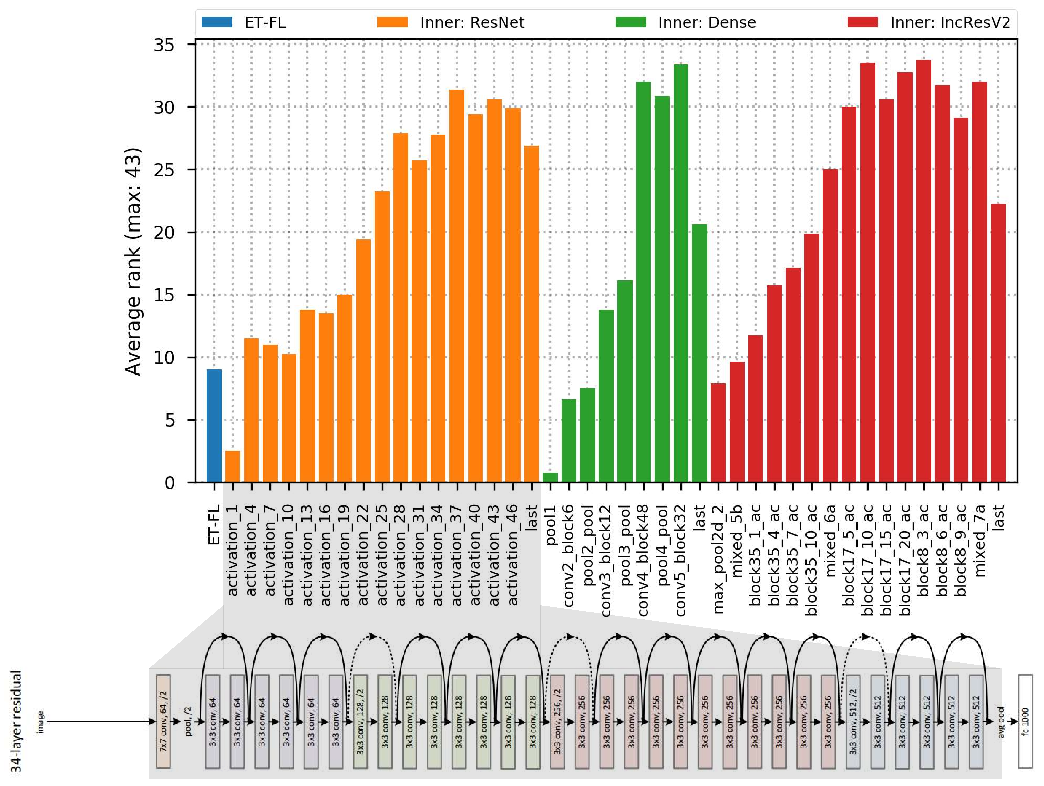
\includegraphics[width=0.7\textwidth]{images/all_per_layer_hori_bars.pdf}
	\end{figure}
	\vfill
\end{frame}


\begin{frame}{Results}
\framesubtitle{More recent networks like DenseNet or ResNet work better}
\begin{figure}
	\center
	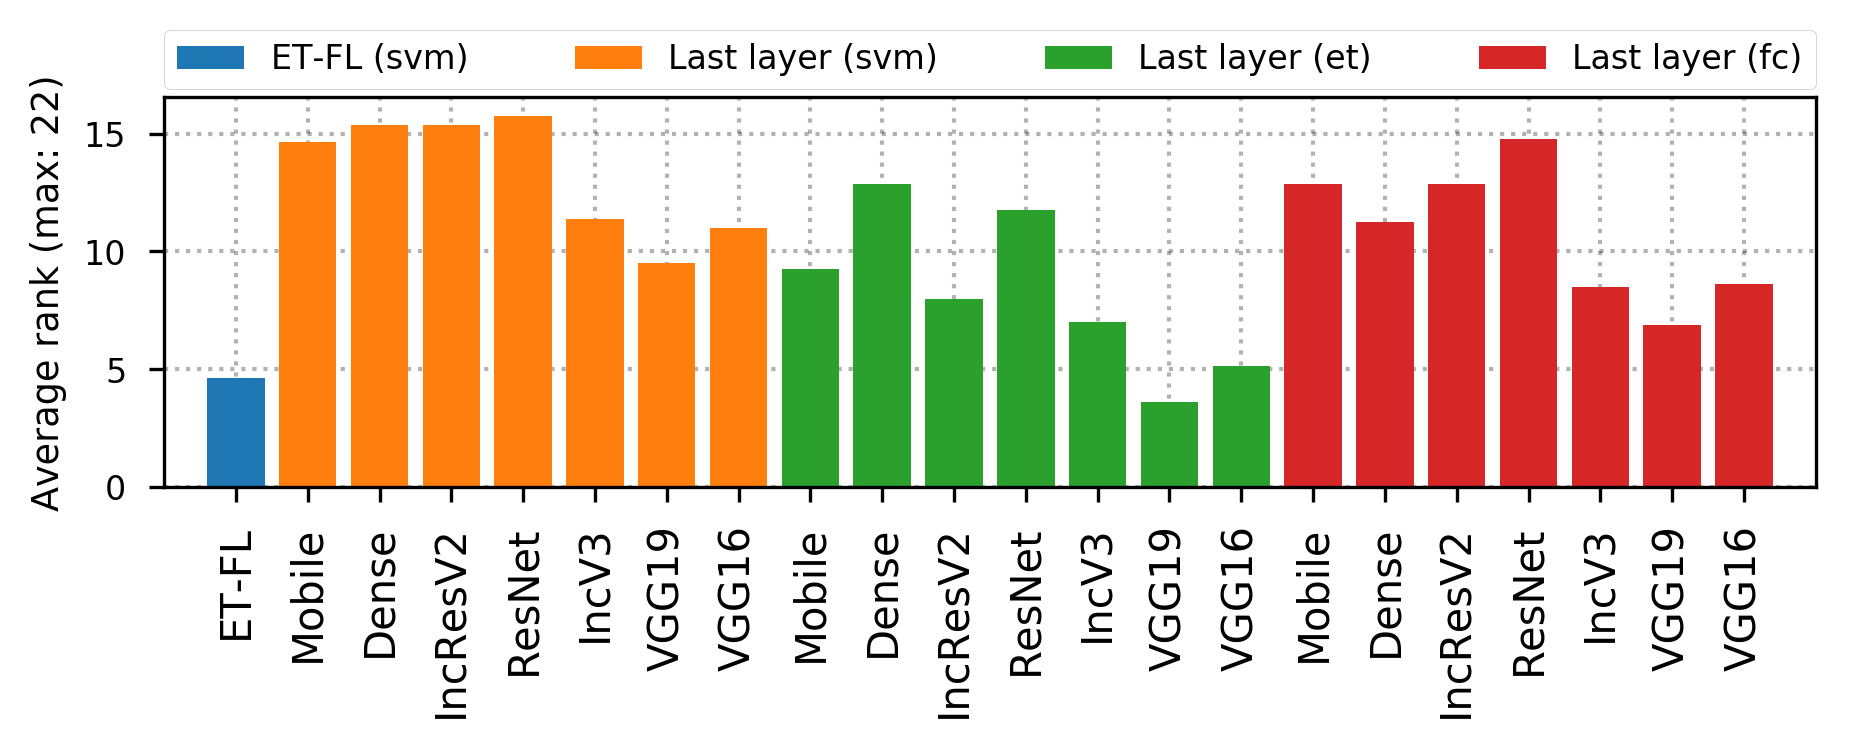
\includegraphics[scale=0.65]{images/last_baseline_bars.png}
\end{figure}

{\footnotesize
	\textbf{See also:} \fullcite{kornblith2019better}
}
\end{frame}

% \begin{frame}{Conclusion}
% 	\vfill
% 	Main {takeaways}:
% 	\vfill
% 	\begin{itemize}
% 		\item {Fine tuning} is the best performing method
% 		\item {Feature extraction} often close to fine-tuning and less computationally expensive
% 		\item Prefer {inner layers feature extraction} to last layers feature extraction
% 		\item Use {more recent networks} such as DenseNet and ResNet
% 	\end{itemize}
% 	\vfill
	
% \end{frame}

\section{Transfer from pathology data}
\subsection{Introduction}

\begin{frame}{}
	\vfill
	\begin{center}
		\Large
		Contribution \#2 \\
		\vspace{0.75cm}
		\textbf{Multi-task pre-training from pathology data} \\
		\vspace{0.75cm}
		{\small (thesis chapter 5)}
	\end{center}
	 
	\vfill

	{
		\footnotesize
		\textbf{Article}: \fullcite{mormont2020multi}
	}	
\end{frame}

\begin{frame}{Using a pathology problem as a source task ?}
	\vfill 
	\textbf{Transfer learning} has been shown to \textbf{work better} when \textbf{target and source tasks are close}. {\tiny \parencite{yosinski2014transferable} }
	\vfill
	Problem: \textbf{no ImageNet-like dataset in pathology} so how can we pre-train a model ? 
	\vfill
	Our proposal: \textbf{multi-task pre-training} with many small datasets rather than a large one. 
	\vfill
\end{frame}

\subsection{Data}
\begin{frame}{Several source tasks}
	\begin{figure}
		\captionsetup{font={tiny}}
    \center
    \begin{subfigure}[t]{0.079\textwidth}
        \centering
        \includegraphics[width=\textwidth]{images/illus/illus_necrose.png}
        \caption{Necrosis}
    \end{subfigure}
    \begin{subfigure}[t]{0.079\textwidth}
        \centering
        \includegraphics[width=\textwidth]{images/illus/illus_patterns.png}
        \caption{ProliferativePattern}
    \end{subfigure}
    \begin{subfigure}[t]{0.079\textwidth}
        \centering
        \includegraphics[width=\textwidth]{images/illus/illus_cells.png}
        \caption{CellInclusion}
    \end{subfigure}
    \begin{subfigure}[t]{0.079\textwidth}
        \centering
        \includegraphics[width=\textwidth]{images/illus/illus_breast.png}
        \caption{Breast}
    \end{subfigure}
    \begin{subfigure}[t]{0.079\textwidth}
        \centering
        \includegraphics[width=\textwidth]{images/illus/illus_glomeruli.png}
        \caption{Glomeruli}
    \end{subfigure}
    \begin{subfigure}[t]{0.079\textwidth}
        \centering
        \includegraphics[width=\textwidth]{images/illus/illus_lbtd_lba.png}
        \caption{MouseLba}
    \end{subfigure}
    \begin{subfigure}[t]{0.079\textwidth}
        \centering
        \includegraphics[width=\textwidth]{images/illus/illus_anapath.png}
        \caption{HumanLba}
    \end{subfigure}
    \begin{subfigure}[t]{0.079\textwidth}
        \centering
        \includegraphics[width=\textwidth]{images/illus/illus_tissus.png}
        \caption{Lung}
    \end{subfigure}
    \begin{subfigure}[t]{0.079\textwidth}
        \centering
        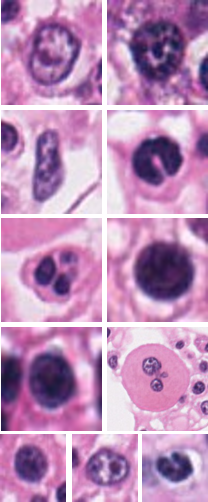
\includegraphics[width=\textwidth]{images/illus/illus_bonemarrow.png}
        \caption{BoneMarrow}
    \end{subfigure}    
    \begin{subfigure}[t]{0.079\textwidth}
        \centering
        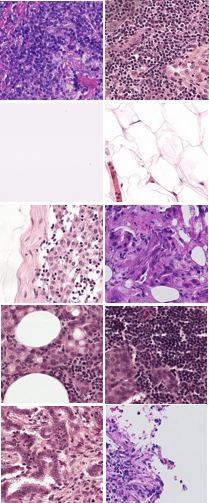
\includegraphics[width=\textwidth]{images/illus/illus_camelyon16.png}
        \caption{Camelyon 16}
    \end{subfigure}
    \begin{subfigure}[t]{0.079\textwidth}
        \centering
        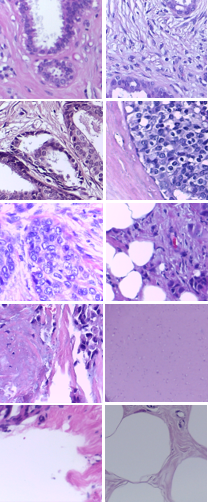
\includegraphics[width=\textwidth]{images/illus/illus_bach18.png}
        \caption{BACH18 Micro}
    \end{subfigure} \\
    \begin{subfigure}[t]{0.079\textwidth}
        \centering
        \includegraphics[width=\textwidth]{images/illus/illus_janowczyk1.png}
        \caption{Janowczyk1}
    \end{subfigure}
    \begin{subfigure}[t]{0.079\textwidth}
        \centering
        \includegraphics[width=\textwidth]{images/illus/illus_janowczyk2.png}
        \caption{Janowczyk2}
    \end{subfigure}
    \begin{subfigure}[t]{0.079\textwidth}
        \centering
        \includegraphics[width=\textwidth]{images/illus/illus_janowczyk5.png}
        \caption{Janowczyk5}
    \end{subfigure}
    \begin{subfigure}[t]{0.079\textwidth}
        \centering
        \includegraphics[width=\textwidth]{images/illus/illus_janowczyk6.png}
        \caption{Janowczyk6}
    \end{subfigure}
    \begin{subfigure}[t]{0.079\textwidth}
        \centering
        \includegraphics[width=\textwidth]{images/illus/illus_janowczyk7.png}
        \caption{Janowczyk7}
    \end{subfigure}
    \begin{subfigure}[t]{0.079\textwidth}
        \centering
        \includegraphics[width=\textwidth]{images/illus/illus_lbpstroma.png}
        \caption{Stroma LBP}
    \end{subfigure}
    \begin{subfigure}[t]{0.079\textwidth}
        \centering
        \includegraphics[width=\textwidth]{images/illus/illus_mitos14.png}
        \caption{MITOS-ATYPIA}
    \end{subfigure}
    \begin{subfigure}[t]{0.079\textwidth}
        \centering
        \includegraphics[width=\textwidth]{images/illus/illus_tupac.png}
        \caption{TUPAC2016 Mitosis}
    \end{subfigure}
    \begin{subfigure}[t]{0.079\textwidth}
        \centering
        \includegraphics[width=\textwidth]{images/illus/illus_umcm.png}
        \caption{UMCM Colorectal}
    \end{subfigure}
    \begin{subfigure}[t]{0.079\textwidth}
        \centering
        \includegraphics[width=\textwidth]{images/illus/illus_warwick.png}
        \caption{Warwick CRC}
    \end{subfigure}
	\end{figure}
\end{frame}

\begin{frame}{Several source tasks}
	\begin{table}[t]
    \centering
    \tiny
    \begin{tabular}{|c|c|c|c|c|}
        \hline
        \textbf{Name} & Organ \& pathology & Stains & Images & Classes \\
        \hline
		Necrosis & breast cancer & IHC & 882 & 2 \\
		Bone marrow & bone marrow & H\&E & 1291 & 9 \\
		ProliferativePattern & thyroid cancer & Diff-Quik & 1857 & 2 \\
		Janowczyk7 & breast, lymphoma & H\&E & 2244 & 3 \\
		Stroma LBP & colorectal cancer & IHC & 2313 & 2 \\
		Warwick CRC & colorectal cancer & H\&E & 2500 & 2 \\
		Janowczyk2 & breast cancer & H\&E & 3402 & 2 \\
		CellInclusion & thyroid cancer & Diff-Quik & 3637 & 2 \\
		MouseLba & lung cancer & MGG & 4284 & 8 \\
		BACH18 Micro & breast cancer & H\&E & 4800 & 4 \\ 
		UMCM Colorectal & colorectal cancer & H\&E& 5000 & 8 \\
		HumanLba & lung cancer & MGG & 5420 & 9 \\
		Lung & lung & H\&E & 6331 & 10 \\
		Breast2 & breast cancer & H\&E & 17523 & 2 \\
		Breast1 & breast cancer & H\&E & 23032 & 2 \\
		Janowczyk5 &  breast cancer & H\&E & 24870 & 2 \\
		Glomeruli & kidney & M3C & 29213 & 2 \\
		Janowczyk1 & breast cancer & H\&E & 31725 & 2 \\
		MITOS-ATYPIA 14 & breast cancer & H\&E & 64873 & 3 \\
		TUPAC2016 Mitosis & breast cancer & H\&E & 77853 & 2 \\
		Janowczyk6 & breast, invasive ductal carci. & H\&E & 277524 & 2 \\
		Camelyon16 & breast cancer & H\&E & 292226 & 2 \\
        \hline 
		
\multicolumn{2}{|c|}{} & \textbf{Total} & {\color{red}\textbf{882800}} & {\color{red}\textbf{81}} \\
\hline
    \end{tabular}
\end{table}
\end{frame}

\subsection{Our approach}
\begin{frame}{Multi-task pre-training architecture}
	Use all source classification tasks simultaneously to train the model.
	\begin{figure}
		\includegraphics[width=\textwidth]{images/multitask-training.pdf}
	\end{figure}
	\begin{itemize}
		\item A shared backbone $\theta_s$ (\textit{e.g.}~: ResNet50, DenseNet121)
		\item A task-specific head $\theta_t$ for each task $t$
		\item Training batch sampling: one batch contains samples from different tasks. 
		\item \textbf{Transfer}: after pre-training, $\theta_s$ can be fine-tuned or used as a feature extractor
	\end{itemize}
\end{frame}

\subsection{Evaluation protocol}
\begin{frame}{Leave-one-task-out}
	We want to evaluate \textbf{how a pre-trained model transfers} to a new unseen task by \textbf{computing a transfer score} (accuracy or ROC AUC). 
	\begin{figure}
		\includegraphics[width=\textwidth]{images/transfer-score-process.pdf}
	\end{figure}
\end{frame}

% \begin{frame}{Evaluation protocol}
% \framesubtitle{Best model selection and evaluation}
% 	\begin{figure}
% 		\includegraphics[width=\textwidth]{images/final-perf-process.pdf}
% 	\end{figure}
% \end{frame}

\subsection{Results}
\begin{frame}{Experiments and results}
\framesubtitle{\textbf{Feature extraction} with multi-task pre-trained models}
\vfill
Compared to ImageNet feature extractors, ours either improve or provide comparable performance.
\vfill
\begin{figure}
	\begin{subfigure}{0.48\textwidth}
		\center
		\includegraphics[width=\textwidth]{images/resnet_fe.png}
		\caption{DenseNet121}
	\end{subfigure}
	\begin{subfigure}{0.48\textwidth}
		\center
		\includegraphics[width=\textwidth]{images/dense_fe.png}
		\caption{ResNet50}
	\end{subfigure}
\end{figure}
\vfill
\end{frame}

\begin{frame}{Results}
	\framesubtitle{\textbf{Fine tuning} with multi-task pre-trained models}
	\vfill
	Compared to fine-tuned ImageNet models, ours provide comparable performance. 
	
	\begin{center}
		Fine-tuning is able to recover lack of specificity of ImageNet features. 
	\end{center}
	
	\vfill
	
	\begin{figure}
		\begin{subfigure}{0.48\textwidth}
			\center
			\includegraphics[width=\textwidth]{images/resnet_ft.png}
			\caption{DenseNet121}
		\end{subfigure}
		\begin{subfigure}{0.48\textwidth}
			\center
			\includegraphics[width=\textwidth]{images/dense_ft.png}
			\caption{ResNet50}
		\end{subfigure}
	\end{figure}
\end{frame}

\begin{frame}{Results}
	\framesubtitle{Comparing to training from scratch and joint training}
	\begin{figure}
		\centering
		\includegraphics[width=\linewidth]{images/joint-banner.pdf}
		\hspace{-0.25cm}
		\caption*{\textit{From scratch - feature extraction - fine-tuning - joint training}}
	\end{figure}

	\begin{itemize}
		\item joint training only improves over fine-tuning on small datasets
		\item fine-tuning outperforms feature extraction {\tiny (contrib. \#1)}
		\item training from scratch is subpar compared to all other approaches
	\end{itemize}

	\begin{figure}
		\begin{subfigure}{\textwidth}
			\centering
			\includegraphics[width=\textwidth]{images/densenet_all.png}
		\end{subfigure}
	\end{figure}

\end{frame}

% \subsection{Conclusion}
% \begin{frame}{Conclusion}
% 	Compared to ImageNet pretrained models, our models:
%  	\begin{itemize}
% 		\item used as \textbf{feature extractors} yield comparable or better performance
% 		\item \textbf{fine-tuned} yield comparable performance
% 	\end{itemize}
% 	\vfill
% 	Also \textbf{training from scratch underperforms} compared to all other evaluated transfer approaches on our tasks.
% \end{frame}

\section{Self-training}
\subsection{Introduction}

\begin{frame}{}
	\vfill
	\begin{center}
		\Large
		Contribution \#3 \\
		\vspace{0.75cm}
		\textbf{Self-training for segmentation from sparsely-labeled data} \\
		\vspace{0.75cm}
		{\small (thesis chapter 6)}
	\end{center}
	 
	\vfill

	{
		\footnotesize
		\textbf{Article}: \fullcite{mormont2022self}
	}	
\end{frame}

\begin{frame}{Thyroid FNAB: an imperfectly-annotated cytology dataset}
	\vfill
	\begin{center}
	A sparsely annotated dataset for thyroid nodule malignancy assessment.
	\end{center}
	\vfill
	\begin{columns}
		\begin{column}[t]{0.48\textwidth}
			\centering
			\includegraphics[width=\textwidth]{images/sparse_thyroid_example1.png}
		\end{column}
		\begin{column}[t]{0.48\textwidth}
			\centering
			\includegraphics[width=\textwidth]{images/sparse_thyroid_example2.png}
		\end{column}
	\end{columns}

	\begin{flushright}
		\tiny
		Annotated by the team of Prof. Isabelle Salmon from Erasme hospital (Université Libre de Bruxelles, BE).
	\end{flushright}
	\vfill
\end{frame}

\begin{frame}{Using sparsely-labeled data}
	\vfill
	\begin{center}
		How to exploit such a sparse/incomplete segmentation dataset in a supervised learning settings ? 
	\end{center}
	\vfill
	\begin{figure}
		\centering
		\includegraphics[height=0.4\textheight]{images/unet.png}
	\end{figure}
	\begin{flushright}
		\tiny \parencite{ronneberger2015unet}
	\end{flushright}
	\vfill
	\textbf{Our proposal}: use the segmentation model being trained to generate the missing information
	\begin{center}
		

		$\Rightarrow$ \textbf{self-training} $\Leftarrow$
	\end{center}
	\vfill
\end{frame}

\begin{frame}[t]{Sparsely-labeled settings}
	\begin{columns}[t]
		\begin{ccolumn}{0.48\textwidth}{$\mathcal{D}_l$ - exhaustively-labeled set}
			\begin{figure}
				\center
				\includegraphics[width=\textwidth]{images/exhaustive_set.png}
			\end{figure}
		\begin{center}
				{\footnotesize $n_l$ images and masks. All pixels have a 0 (background) or 1 (foreground) label.}
		\end{center}
		\end{ccolumn}
		% --------------------------
		\begin{ccolumn}{0.48\textwidth}{$\mathcal{D}_s$ - sparsely-labeled set}
			\begin{figure}
				\center
				\includegraphics[width=\textwidth]{images/sparse_set.png}
			\end{figure}
		\begin{center}
				{\footnotesize $n_s$ images and masks. Unlabeled pixels have label 0 (background) and labeled pixels are exclusively foreground.}
		\end{center}
		\end{ccolumn}
	\end{columns}
	\vfill
\end{frame}

\subsection{Our algorithm}
\begin{frame}{Our self-training algorithm}
	\begin{figure}
		\centering
		\includegraphics[width=\textwidth]{images/selftrain-algo.png}
	\end{figure}
\end{frame}

\begin{frame}{Weighting startegies}

	We \textbf{weigh the pixel contribution} in the loss:
	\[
		\mathcal{L} = \frac{1}{|\mathbf{y}|}\sum_{i}\sum_{j} w_{ij} \ell(\hat{y}_{ij}; y_{ij}) 
	\] 
	For instance:
	\begin{itemize}
		\item \textbf{Constant}: $w^{(cst)}_{ij} = C > 0$ where $C$ is an hyperparameter
		\item \textbf{Entropy}: $w^{(ent)}_{ij}$ is the entropy of the model prediction $\hat{y}_{ij}$
	\end{itemize}
	%Eventually, $w_{ij}$ is obtained by normalizing the weights computed over a patch so that they sum to 1.
\end{frame}

% \begin{frame}{Pseudo-labeling: hard \textit{vs.} soft}
% 	Generating a pseudo-label $y^{({pl})}_{ij}$ for a pixel from the model prediction $\hat{y}_{ij}$ for this pixel:
% 	\[
% 		y^{({pl})}_{ij} = \begin{cases}
% 			1,\,\text{if}\, y_{ij} = 1 \\
% 			g(\hat{y}_{ij}),\,\text{otherwise}
% 		\end{cases}
% 	\]

% 	\begin{columns}
% 		\begin{ccolumn}{0.48\textwidth}{Soft labeling}
% 			\tiny
% 			Use the sigmoid output of the model as-is:
% 			\[
% 				g(x) = x
% 			\]
% 			The pseudo-label can be seen as a probability in $\left]0,1\right[$ .
% 		\end{ccolumn}
% 		\begin{ccolumn}{0.48\textwidth}{Hard labeling}
% 			\tiny
% 			Binarize the model output with a threshold:
% 			\[
% 				g(x) = \begin{cases}
% 				1,\,\text{if}\, x > T_e\\
% 				0,\,\text{otherwise}
% 				\end{cases}
% 			\]
% 			% Determine the threshold by optimizing the Dice coefficient on the exhaustively-labeled set $\mathcal{D}_l$: 
% 			% \begin{align*}
% 			% Dice_T(\mathbf{y},\hat{\mathbf{y}}) = \dfrac{2 \times \sum_{i,j} \left[\mathbb{1}_{\hat{y}_{ij} \geq T} \times y_{ij}\right]}{\sum_{i,j} \mathbb{1}_{\hat{y}_{ij} \geq T} + \sum_{i,j} y_{ij}} \\
% 			% T_e = \arg \underset{T}{\max} \sum_{(\mathbf{x}, \mathbf{y}) \in \mathcal{D}_l} \text{Dice}_T\left(\mathbf{y},h( \mathbf{x}; \theta_{e})\right)
% 			% \end{align*}
		
% 		\end{ccolumn}
% 	\end{columns}
% \end{frame}

% \begin{frame}{Weighting strategies}
% 	We weight the pixel contribution in the loss:
% 	\[
% 		\mathcal{L} = \frac{1}{|\mathbf{y}|}\sum_{i}\sum_{j} w_{ij} \ell(\hat{y}_{ij}; y_{ij}) 
% 	\] 
% 	The weighting strategy is an hyperparameter:
% 	\begin{itemize}
% 		\item \textbf{Constant}: $w^{(cst)}_{ij} = C > 0$ where $C$ is an hyperparameter
% 		\item \textbf{Entropy}: $w^{(ent)}_{ij}$ is the entropy of the model prediction $\hat{y}_{ij}$
% 		\item \textbf{Consistency}: $w^{(cty)}_{ij}$ is a consistency score between model predictions of pixel $(i,j)$ and close pixels
% 		\item \textbf{Merged}: $w^{(mgd)}_{ij}$ combines the \textit{entropy} and \textit{consistency} strategies
% 	\end{itemize}
% 	Eventually, $w_{ij}$ is obtained by normalizing the weights computed over a patch so that they sum to 1.
% \end{frame}

\subsection{Experiments}
\begin{frame}{Experiments}
\framesubtitle{3 public datasets}
	\centering
	\begin{columns}
		\begin{ccolumn}{0.30\textwidth}{MoNuSeg}
			\centering \includegraphics[width=\textwidth]{images/monuseg_rep.png}
			\begin{raggedright} \tiny \parencite{kumar2019multi} \end{raggedright}
		\end{ccolumn}
		% --------------------------
		\begin{ccolumn}{0.30\textwidth}{SegPC}
			\centering \includegraphics[width=\textwidth]{images/segpc_rep.png}
			\begin{raggedright} \tiny \parencite{gupta2021segpc} \end{raggedright}
		\end{ccolumn}
		% --------------------------
		\begin{ccolumn}{0.30\textwidth}{GlaS}
			\centering \includegraphics[width=\textwidth]{images/glas_rep.png}
			\begin{raggedright} \tiny \parencite{sirinukunwattana2017gland} \end{raggedright}
		\end{ccolumn}
	\end{columns}
	\vfill
	Sparsity is simulated by randomly removing $\rho \%$ of annotations in $n_s$ images.
	\vfill
\end{frame}

\begin{frame}{Experiments}
\framesubtitle{3 baselines}
	\vfill
	\begin{columns}[t]
		\begin{ccolumn}{0.30\textwidth}{(1) $|\mathcal{D}_s| = 0$ }
			\begin{figure} \centering \includegraphics[height=0.3\textheight]{images/baseline1.png} \end{figure}%
\vspace{-0.8cm}
\begin{flushright}{\tiny (orignal dataset)}\end{flushright}
		\end{ccolumn}
		\begin{ccolumn}{0.30\textwidth}{(2) $\mathcal{D}_l$ only}
			\begin{figure} \centering \includegraphics[height=0.3\textheight]{images/baseline2.png} \end{figure}
		\end{ccolumn}
		\begin{ccolumn}{0.30\textwidth}{(3) $\mathcal{D}_l \cup \mathcal{D}_s$}
			\begin{figure} \centering \includegraphics[height=0.3\textheight]{images/baseline3.png} \end{figure}%
\vspace{-0.5cm}
\begin{raggedright}{\tiny (unlab. pixels assigned to background)}\end{raggedright}%
		\end{ccolumn}
	\end{columns}
	\vfill
	\begin{center}
		To be considered of interest, our method should be as close as possible to (1) (upper bound) and outperform baselines (2) and (3).
	\end{center}
	\vfill
\end{frame}

\subsection{Results}
% \begin{frame}{Results}
% \framesubtitle{Hard vs. soft labeling}
% 	\vfill
% 	For the given data scarcity regime ($\rho = 90\%$):
% 	\begin{itemize}
% 		\item The best performance are obtained with hard labels.  
% 		\item Soft labeling yields more stability as performance are less impacted by the choice of a weighting strategy  
% 	\end{itemize}

% 	\vfill

% 	\begin{figure}
% 		\centering
% 		\includegraphics[width=\textwidth]{images/plot_hard_vs_soft_test_pxl_self_hard_dice.pdf}
% 	\end{figure}
% \end{frame}

\begin{frame}{Results}
\framesubtitle{Self-training at fixed $n_l$ - MoNuSeg}
	\vfill
	\begin{itemize}
		\item There is always a cut-off point at which \textbf{exploiting additional sparse annotations with self-training becomes beneficial} !
		\item Self-training struggles at very high data scarcity
		\item Using $\mathcal{D}_s$ as if it was exhaustively annotated is a bad idea
	\end{itemize}
	\begin{center}
		For MoNuSeg, the upper baseline is reached with only $\sim 30\%$ of the original annotations. \\
	\end{center}	
	\vfill
	\begin{figure}
		\centering
		\includegraphics[width=\textwidth]{images/monuseg_test_pxl_self_hard_dice_rho.pdf}
	\end{figure}
\end{frame}


% \begin{frame}{Results}
% 	\framesubtitle{Self-training at fixed $n_l$ - SegPC and GlaS}
% 	\begin{figure}
% 		\begin{subfigure}{\textwidth}
% 			\centering
% 			\caption{Glas}
% 			\includegraphics[width=\textwidth]{images/glas_test_pxl_self_hard_dice_rho.pdf}
% 		\end{subfigure}
% 		\begin{subfigure}{\textwidth}
% 			\centering
% 			\caption{SegPC}
% 			\includegraphics[width=\textwidth]{images/segpc_test_pxl_self_hard_dice_rho.pdf}
% 		\end{subfigure}
% 	\end{figure}
% \end{frame}

% \begin{frame}{Results}
% \framesubtitle{Label sparsely or exhaustively ?}
% 	\begin{itemize}
% 		\item The answser is dataset-dependant !
% 		\item MoNuSeg: annotation budget better spent on sparse labeling (later used with self-training)
% 		\item Others: annotation better spent on exhaustive labeling and using supervised training
% 	\end{itemize}
% 	\begin{figure}
% 		\centering
% 		\begin{subfigure}{0.32\textwidth}
% 			\includegraphics[width=\textwidth]{images/annot_strat_monuseg.pdf}
% 			\caption{MoNuSeg}
% 		\end{subfigure}
% 		\begin{subfigure}{0.32\textwidth}
% 			\includegraphics[width=\textwidth]{images/annot_strat_glas.pdf}
% 			\caption{GlaS}
% 		\end{subfigure}
% 		\begin{subfigure}{0.32\textwidth}
% 			\includegraphics[width=\textwidth]{images/annot_strat_segpc.pdf}
% 			\caption{SegPC}
% 		\end{subfigure}
% 	\end{figure}
% \end{frame}

\begin{frame}{Results}
\framesubtitle{Application to Thyroid FNAB}

\vfill
\begin{center}
	Self-training significantly outperforms the ``$\mathcal{D}_l$ only'' and ``$\mathcal{D}_l \cup \mathcal{D}_s$'' baselines.
\end{center}

\vfill
\begin{table}[t]
  \centering 
  \begin{tabular}{|c|c|}
    \hline
    Method & $\text{Dice}^*$ (\%)\\
    \hline
    Self-training & $89.05 \pm 0.85$ \\
    $\mathcal{D}_l$ only & $80.30 \pm 5.39$\\  
    $\mathcal{D}_l \cup \mathcal{D}_s$ & $83.62 \pm 3.52$\\
    \hline
  \end{tabular}
\end{table}
\vfill

\begin{figure}
	\centering
	\begin{subfigure}{0.32\textwidth}
		\centering
		\includegraphics[width=\textwidth]{images/thyroid_wsi_example1.png}	
	\end{subfigure}
	\begin{subfigure}{0.32\textwidth}
		\centering
		\includegraphics[width=\textwidth]{images/thyroid_wsi_example2.png}	
	\end{subfigure}
	\begin{subfigure}{0.32\textwidth}
		\centering
		\includegraphics[width=\textwidth]{images/thyroid_wsi_example3.png}	
	\end{subfigure}
\end{figure}
\end{frame}


\begin{frame}{Conclusion}
	\begin{itemize}
		\item Self-training can be used to obtain competitive segmentation performance with less annotations !
		\item Some datasets might benefit more from sparse labeling then exhaustive labeling
	\end{itemize}
	\vfill
	Future works:
	\begin{itemize}
		\item From binary to multi-class segmentation
		\item How does the type of dataset impact the performance ?
		\item Study the interest of the method in low scarcity conditions
	\end{itemize}
\end{frame}

\section{Conclusion of the thesis}
\begin{frame}{Conclusion of the thesis}
	\vfill
	\begin{exampleblock}{}
		Data scarcity in digital pathology is not an inextricable issue and there exists algorithmic solutions to at least alleviate it.
	\end{exampleblock}
	\vfill
	\begin{itemize}
		\item \textbf{Transfer learning} is an effective approach: feature extraction is a strong baseline, fine-tuning is better
		\item \textbf{Multi-task pre-training} is a viable strategy to pre-train a model on pathology data
		\item \textbf{Self-training} with sparsely-labeled datasets can be used to cut down the dataset size requirements for training a segmentation model 
	\end{itemize}
	\vfill
\end{frame}

\section{Future works}
\begin{frame}{Perspectives}
	\begin{itemize}
		\item Transfer learning with new architectures 
		\item Consider more tasks and type of tasks (\textit{e.g.}~ detection, segmentation)
		\item Self-training as an interactive annotation algorithm
		\item Systematic benchmarking of representation learning in pathology
	\end{itemize}
\end{frame}

\begin{frame}{Self-trained model integration in a workflow}
	Workflow to detect atypical cells.  
	\begin{figure}
		\includegraphics[width=\textwidth]{images/pipeline.pdf}		
	\end{figure}
\end{frame}

\begin{frame}
	\vfill
	{\Large Thank you !}
	\vfill
\end{frame}

%\begin{frame}{Deep learning}
%\vspace*{-0.5cm}
%\begin{columns}
%%
%   \begin{ccolumn}{0.48\textwidth}{blue}{Training from scratch}
%   		Initialize weights randomly and train as usual.
%        \begin{itemize}
%			\item[$-$] Needs lots of data
%			\item[$-$] Needs much computing resources 
%		\end{itemize}
%    \end{ccolumn}
%
%
%\end{columns}
%\begin{columns}
%
%	\begin{ccolumn}{0.48\textwidth}   {red}{Off-the-shelf}
%		Use pre-trained weight, then use features off-the-shelf.
%		\begin{itemize}
%			\item[$+$] Needs less data then training from scratch
%			\item[$+$] Needs less computing resources 
%		\end{itemize}
%	\end{ccolumn}
%
%
%
%	\begin{ccolumn}{0.48\textwidth}{green}{Fine-tuning}
%		Initialize with pre-trained weigths, and train for few epochs.
%		\begin{itemize}
%			\item[$+$] Needs less data than training from scratch
%			\item[$-$] Needs much computing resources 
%		\end{itemize}
%	\end{ccolumn}
%
%\end{columns}	
%
%\end{frame}
%\begin{frame}{Deep transfer learning: how to ?}
%\textbf{Aim}: evaluate which \textbf{deep transfer learning} strategy yields best results using the 8 datasets.
%
%\begin{itemize}
%	\item Deep learning works well with images 
%	\item Transfer learning usually requires less data and computing resources {\color{red} (cite)}
%	\item DTL has been applied to biomedical problems since 2015 {\color{red} (cite)}
%\end{itemize} 
%
%But... \textbf{few people have actually studied how DTL should be applied} !
%
%\begin{itemize}
%	\item most publications use "old" networks (AlexNet, VGGs, GoogLeNet,...)
%	\item studies which do are often too small scale to draw general conclusions 
%\end{itemize}
%\end{frame}
%
%\begin{frame}{Framework}
%\begin{figure}
%	\includegraphics[scale=0.35]{images/offtheshelf_schema.png}
%\end{figure}
%\end{frame}
%
%\begin{frame}{Transfer strategies}
%\begin{columns}
%
%\begin{column}{0.31\textwidth} 
%	\begin{orangebox}{Last layer features}
%		
%	\end{orangebox}
%\end{column}
%
%\begin{column}{0.31\textwidth} 
%	\begin{greenbox}{Feature selection}
%		
%	\end{greenbox}
%\end{column}
%
%\begin{column}{0.31\textwidth}
%	\begin{redbox}{Merging models}
%		
%	\end{redbox} 
%\end{column}
%
%\end{columns}
%
%\begin{columns}
%
%\begin{column}{0.31\textwidth} 
%	\begin{purplebox}{Merging networks}
%		
%	\end{purplebox}
%\end{column}
%
%\begin{column}{0.31\textwidth} 
%	\begin{brownbox}{Fine-tuning}
%		
%	\end{brownbox}
%\end{column}
%
%\begin{colorbox}{0.31\textwidth}{bluebox}{Inner layers}
%\end{colorbox}
%
%\end{columns}
%\end{frame}

\begin{frame}{Pseudo-labels}
	\textbf{Generating a pseudo-label} $y^{({pl})}_{ij}$ for an unlabeled pixel from the model prediction $\hat{y}_{ij}$ for this pixel:
	\begin{itemize}
		\item Soft label: use $\hat{y}_{ij}$ as-is 
		\item Hard label: 1 if $\hat{y}_{ij} > T$, 0 otherwise. $T$ is an auto-calibrated threshold. 
	\end{itemize}
\end{frame}
\end{document}
